\graphicspath{{./images/bmps/}{./images/vects/}{./images/}
  {./images/presentation/bmps/}{./images/presentation/vects/}{./images/presentation/}
  {./images/chapter00/bmps/}{./images/chapter00/vects/}{./images/chapter00/}
  {./images/chapter01/bmps/}{./images/chapter01/vects/}{./images/chapter01/}
  {./images/chapter02/bmps/}{./images/chapter02/vects/}{./images/chapter02/}
  {./images/chapter03/bmps/}{./images/chapter03/vects/}{./images/chapter03/}
  {./images/chapter04/bmps/}{./images/chapter04/vects/}{./images/chapter04/}
  {./images/chapter05/bmps/}{./images/chapter05/vects/}{./images/chapter05/}
  {./images/chapter06/bmps/}{./images/chapter06/vects/}{./images/chapter06/}
  {./images/chapter07/bmps/}{./images/chapter07/vects/}{./images/chapter07/}}
  
\subsection{Change Detection for Obstacle Localization in Images}

\begin{frame}{Sequence example}
  \begin{figure}[h!]
      \centering
      \begin{subfigure}[b]{0.24\columnwidth}
	  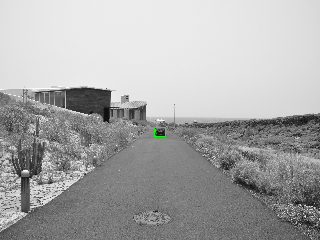
\includegraphics[width=\textwidth]{sequence/seq1}\label{fig:seq1}
      \end{subfigure}% 
      ~
      \begin{subfigure}[b]{0.24\columnwidth}
	  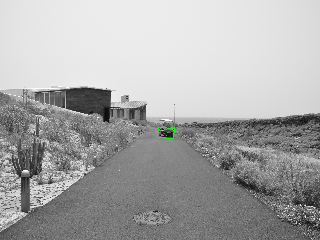
\includegraphics[width=\textwidth]{sequence/seq2}\label{fig:seq2}
      \end{subfigure}%       
      ~
      \begin{subfigure}[b]{0.24\columnwidth}
	  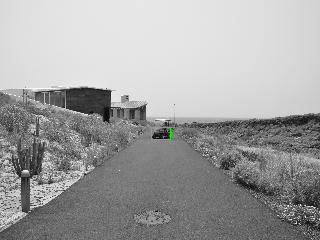
\includegraphics[width=\textwidth]{sequence/seq3}\label{fig:seq3}
      \end{subfigure}%    
      ~
      \begin{subfigure}[b]{0.24\columnwidth}
	  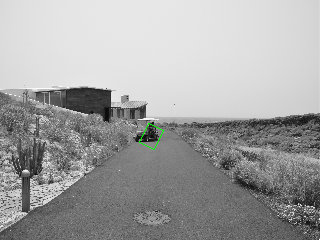
\includegraphics[width=\textwidth]{sequence/seq4}\label{fig:seq4}
      \end{subfigure}%
      \\
      \begin{subfigure}[b]{0.24\columnwidth}
	  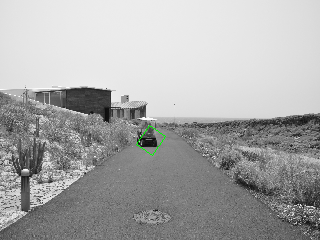
\includegraphics[width=\textwidth]{sequence/seq5}\label{fig:seq5}
      \end{subfigure}% 
      ~
      \begin{subfigure}[b]{0.24\columnwidth}
	  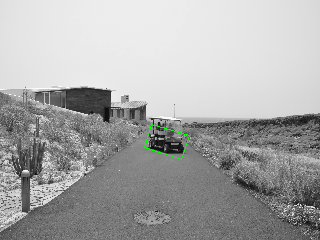
\includegraphics[width=\textwidth]{sequence/seq6}\label{fig:seq6}
      \end{subfigure}%       
      ~
      \begin{subfigure}[b]{0.24\columnwidth}
	  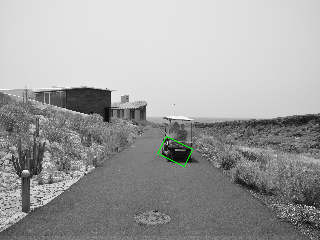
\includegraphics[width=\textwidth]{sequence/seq7}\label{fig:seq7}
      \end{subfigure}%    
      ~
      \begin{subfigure}[b]{0.24\columnwidth}
	  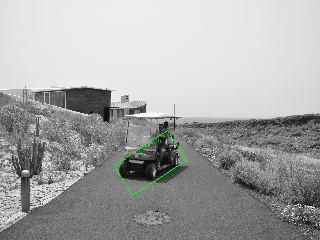
\includegraphics[width=\textwidth]{sequence/seq8}\label{fig:seq8}
      \end{subfigure}%
  \end{figure}
\end{frame}

\subsection{Non-Rigid Contour Tracking}

\begin{frame}{Evaluation method}
  \begin{itemize}
  \only<1>{
   \item We compare three methods:
   \begin{itemize}
    \item BCCPDI-CPD (our method).
    \item Optical flow based method.
    \item Kinect based OpenNI method.
   \end{itemize}
   \item Initial configuration provided by Kinect.
   }
   \only<2> {
   \item For each joint $s_i$ in the skeleton $S$,
   \begin{enumerate}
    \item Generation of set $\mathcal{D} = \{ x \in X \cup s_i \}$
    \item Delaunay triangulation (visibility graph).
    \item Based on the correspondences obtained, we solve
   \end{enumerate}
    \begin{minipage}[c]{\textwidth}
      \tiny
      \begin{equation}\nonumber
	\left( \begin{array}{cc}
	  1 & x'_0 \\
	  \vdots & \vdots \\
	  1 & x'_k \\
	  \vdots & \vdots \\
	  1 & x'_K \end{array} \right)
	    \left( \begin{array}{c}
	  s'_i(x) \\
	  1 \end{array} \right) = 
	    \left( \begin{array}{cc}
	  d_0 \\
	  \vdots \\
	  d_k \\
	  \vdots \\
	  d_K \end{array} \right)
      \end{equation}
    \end{minipage}
%     \vskip-5cm
    \begin{figure}
        \centering
        \begin{subfigure}[b]{0.3\textwidth}
                \centering
                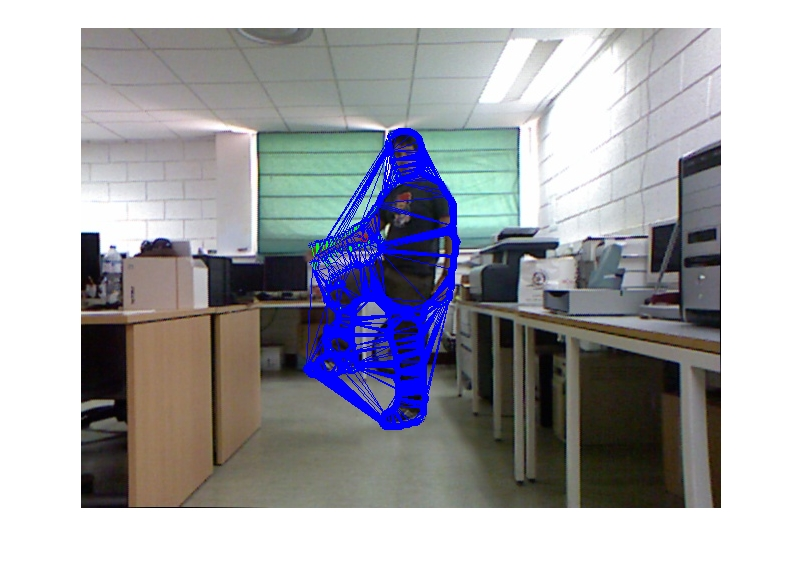
\includegraphics[width=\textwidth, trim=0 0 0 0,clip]{fig21.jpg}
%                 \caption*{Triangulation}
        \end{subfigure}%
	 ~
        \begin{subfigure}[b]{0.3\textwidth}
                \centering
                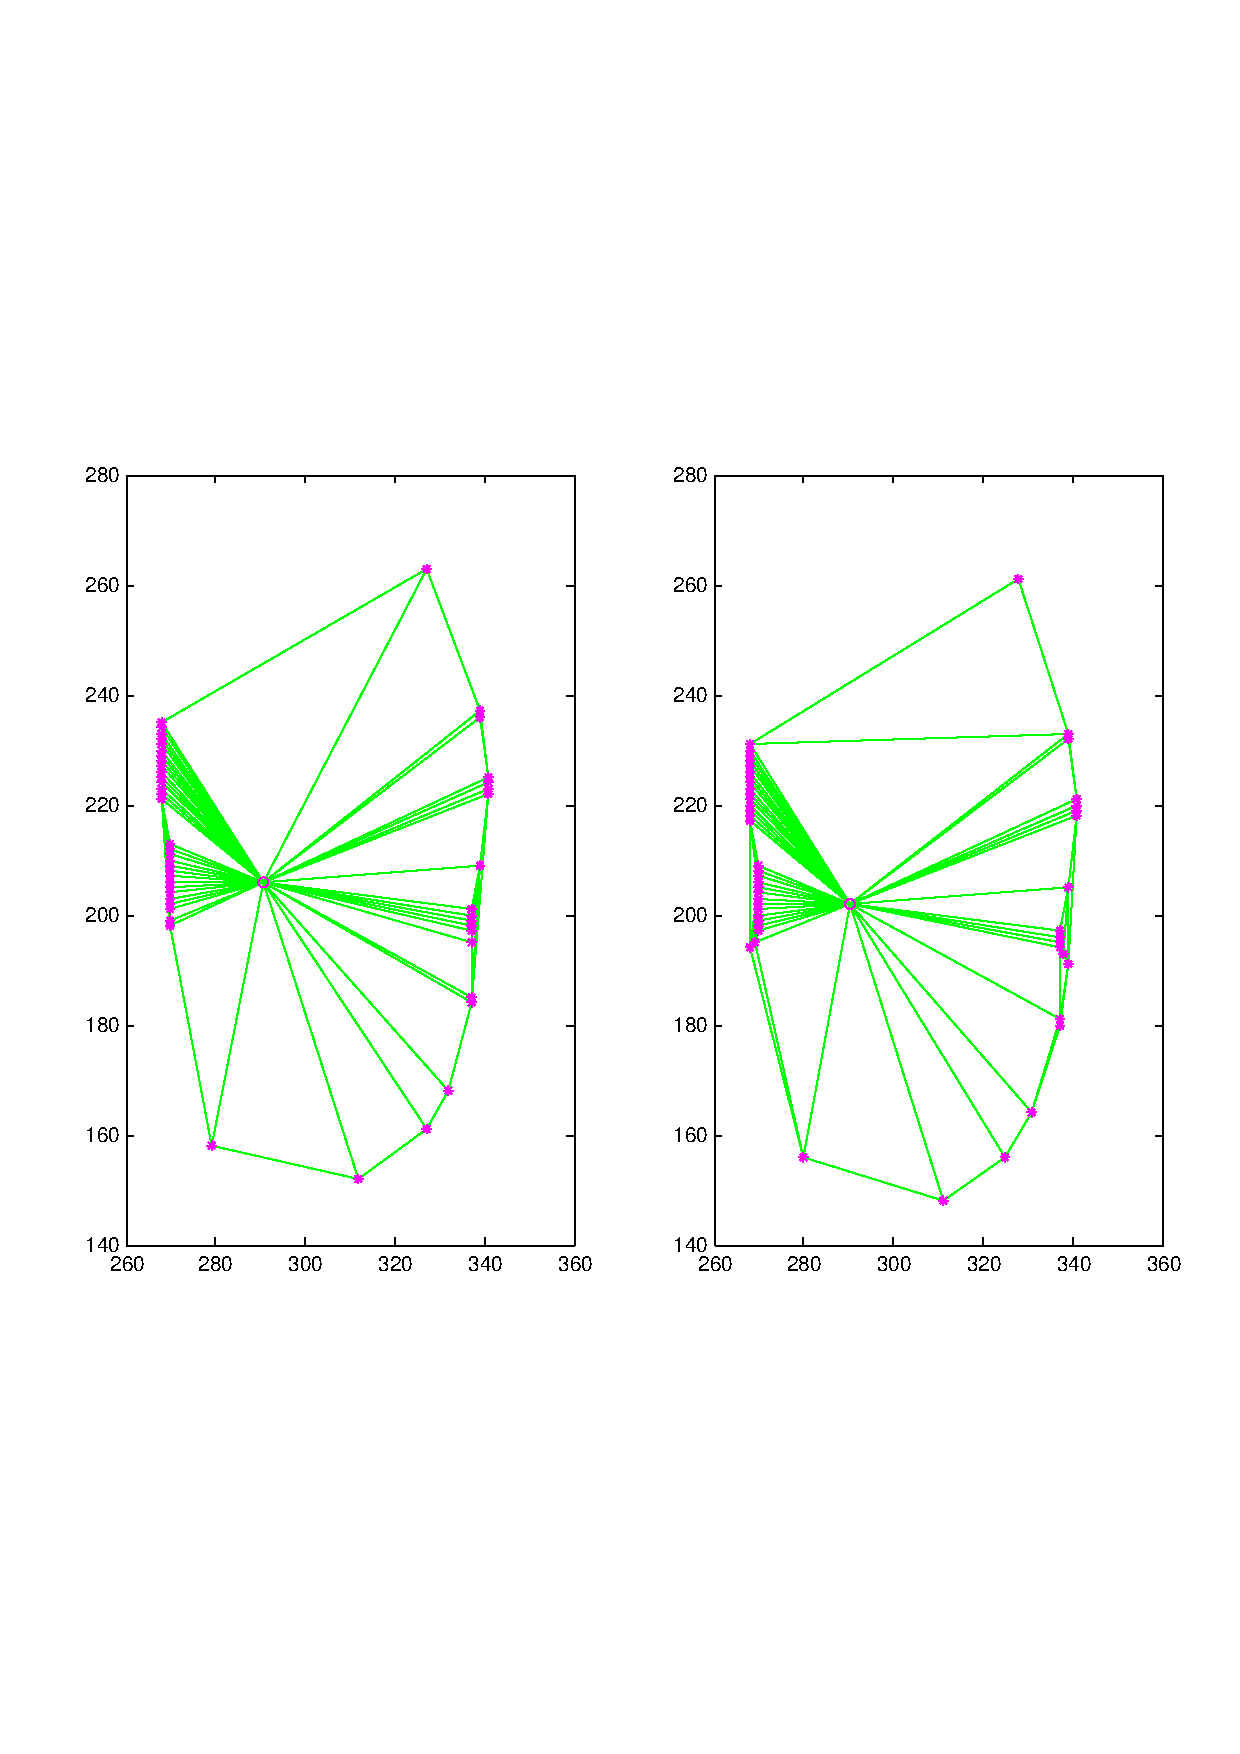
\includegraphics[width=\textwidth, trim=40 230 30 220,clip]{fig22.pdf}
%                 \caption*{Trilateration}
        \end{subfigure}%
        ~
        \begin{subfigure}[b]{0.3\textwidth}
                \centering
                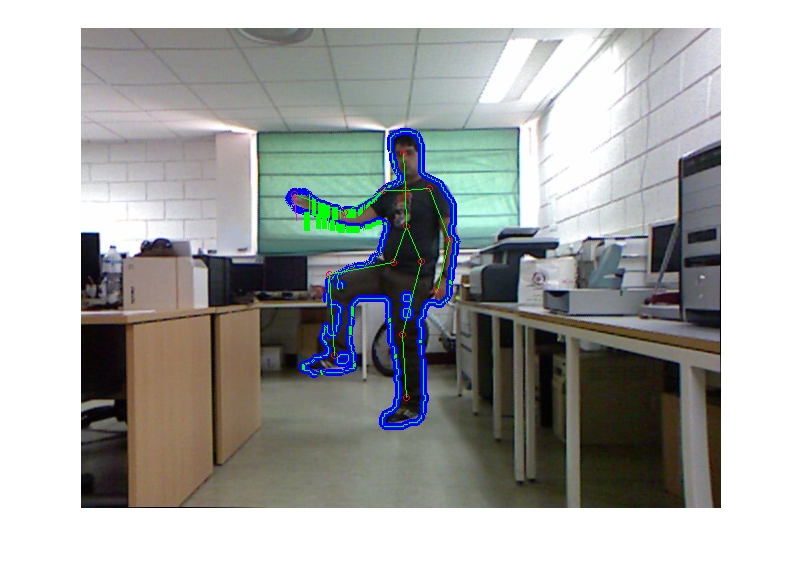
\includegraphics[width=\textwidth, trim=0 0 0 0,clip]{fig23.jpg}
%                 \caption*{New joints}
        \end{subfigure}%      
    \end{figure}
   }


  \end{itemize}
  
  \note {
  \begin{itemize}
   \item For each frame at time $t$, we have an initial skeleton provided by the Kinect, which is used as the initial configuration. From this skeleton, we repeat the following process for each joint $s_i$ in the skeleton $S$
   \item First, we look for the joint nearest points in the contour of the silhouette. To do that, we create the set of points $\mathcal{D} = \{ x \in X \cup s_i \}$, and a Delaunay triangulation is applied to them. This triangulation can be thought also as a visibility graph in which we will select the subset of points $X' \subseteq X$ for which all the points in $X'$ have a connection with the joint $s_i$. This idea is represented in the left image of figure \ref{fig:cp02_err_measure_trilateration}. For each point in $X'$, we also obtain the set $D = \{ x'_k - s_i) | x'_k \in X' \} $.
  \item For each $x'_k \in X'$, we obtain the set of correspondences $Y' \subseteq Y$ at the new frame $t + 1$, 
  obtained using the CPD algorithm. Using this new set and $D$, we can obtain the new position $s'_i$ by 
  trilateration. As we are working in 2D, in this case we can separate the $x$ and $y$ components in order to have two 
  separate linear problems for which we have one variable and more than one equation. For instance, we solve the following system of equations to obtain the value of $s'_i(x)$:
  \end{itemize}
  }

\end{frame}

\begin{frame}[plain]{Final algorithm evaluation}
  \framesubtitle{Displacement comparison}
  \begin{center}
  \begin{figure}
        \centering

        \begin{subfigure}[b]{0.5\columnwidth}
                \centering
                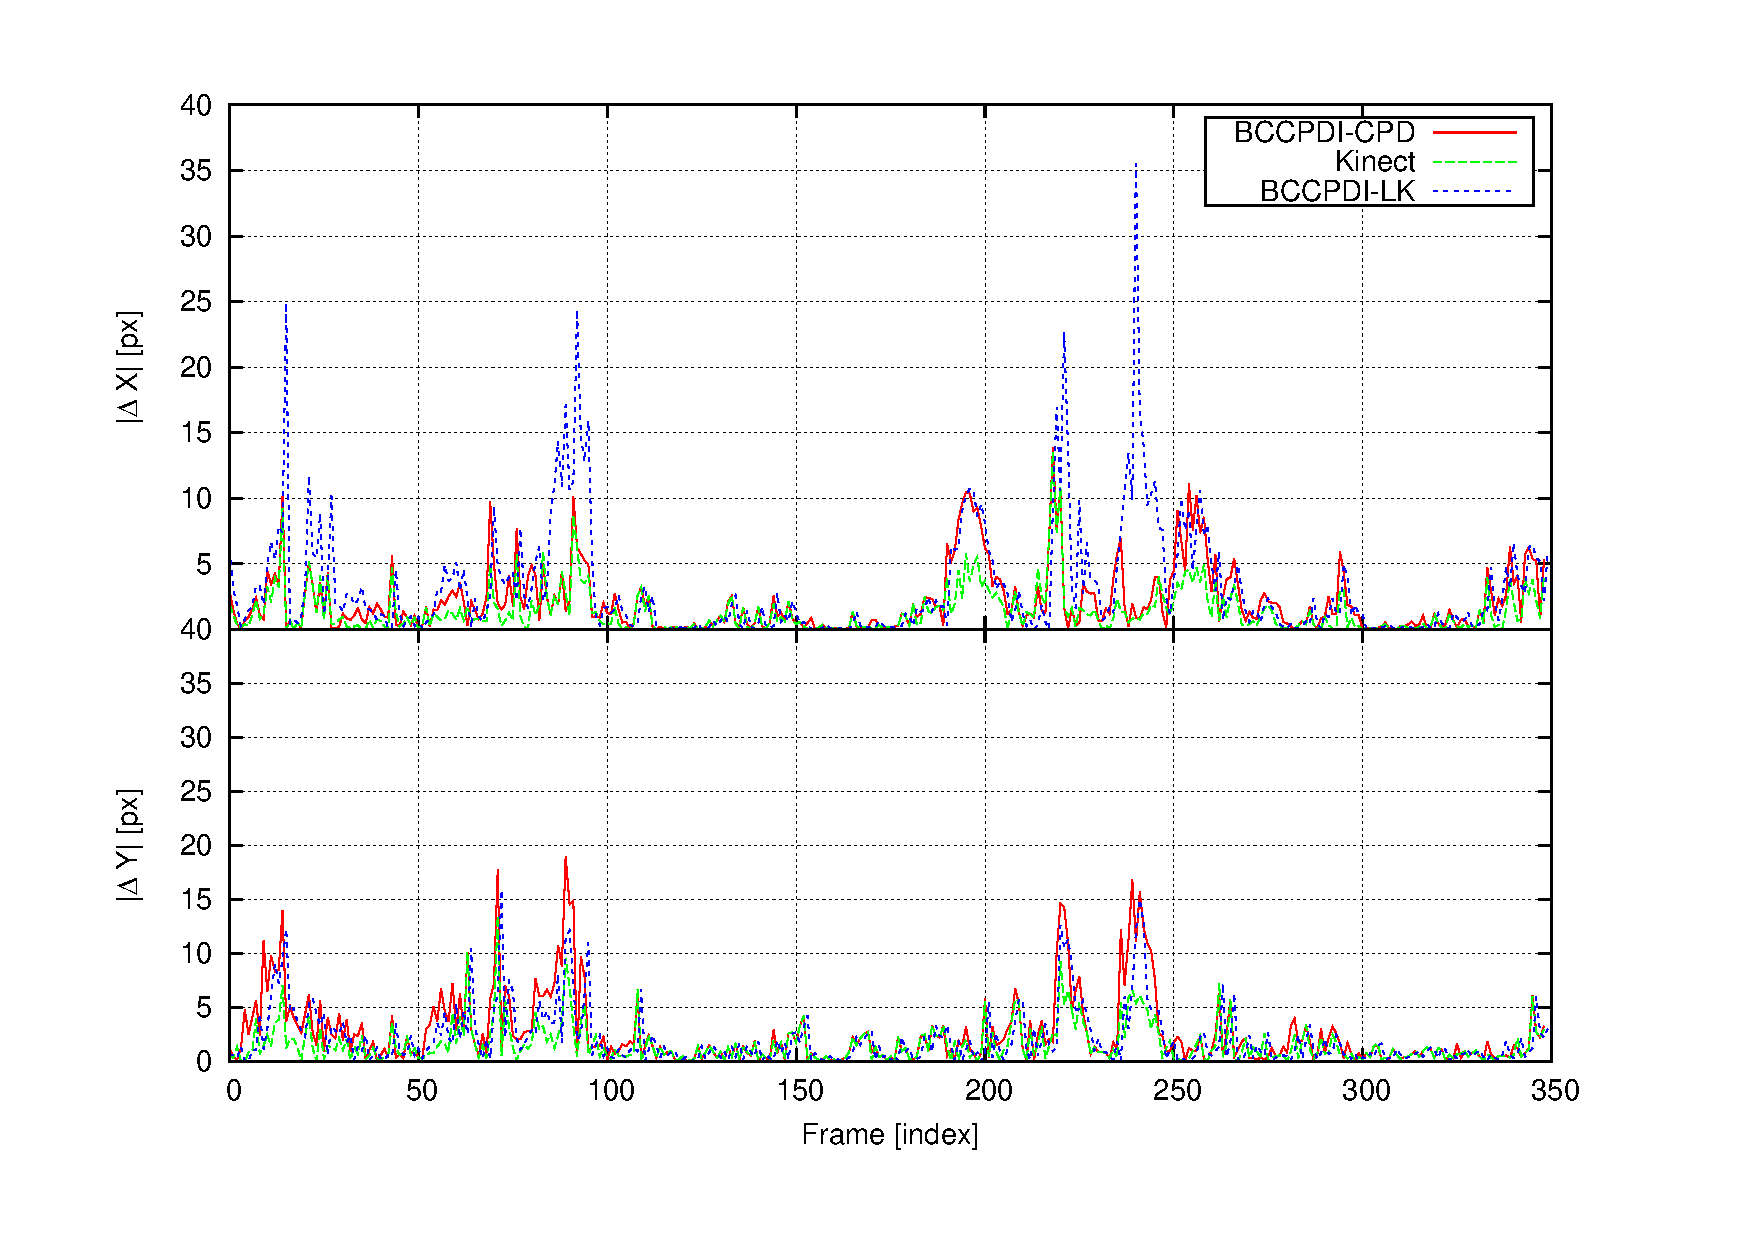
\includegraphics[width=\textwidth, trim=50 40 80 40,clip]{fig27.pdf}
                \caption*{Left elbow}
        \end{subfigure}%        
        \begin{subfigure}[b]{0.5\columnwidth}
                \centering
		  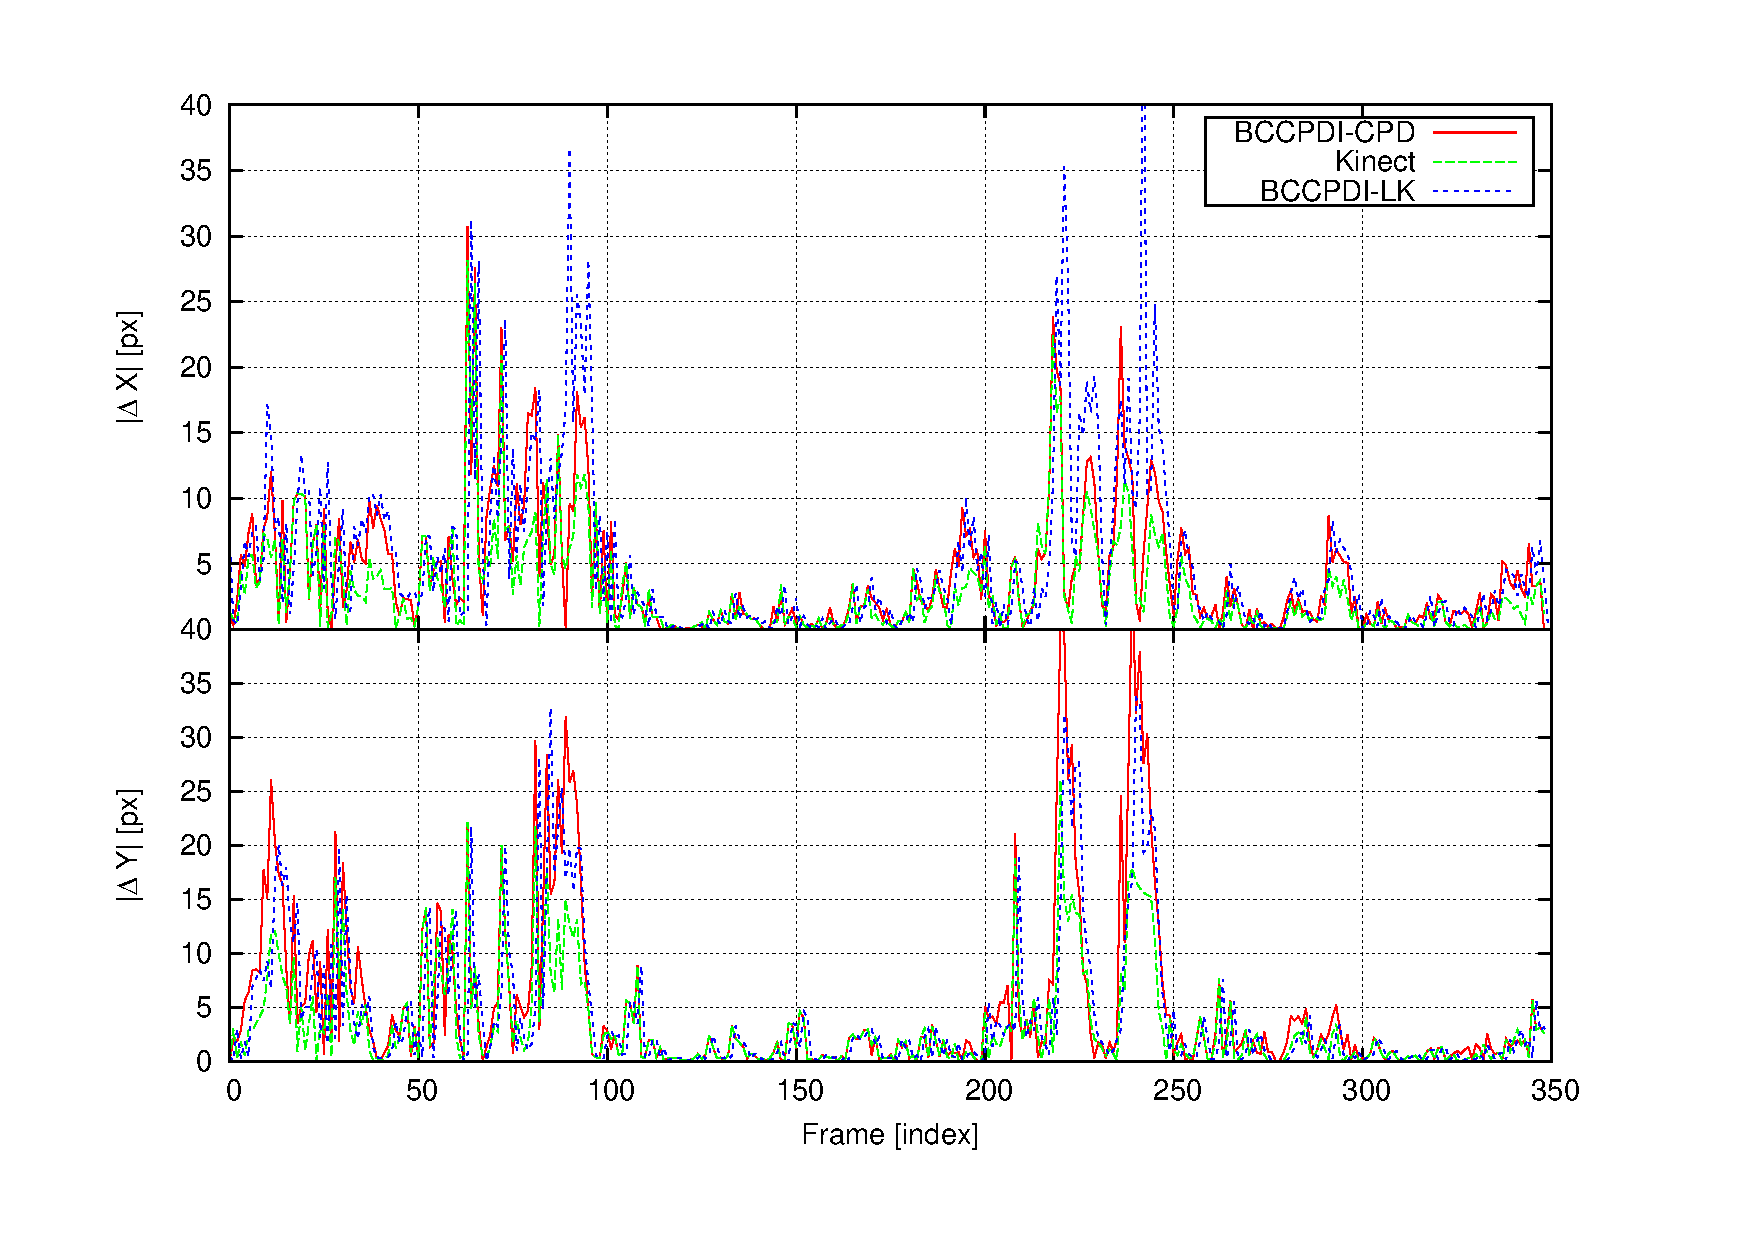
\includegraphics[width=\textwidth, trim=50 40 80 40,clip]{fig28.pdf}
                \caption*{Left hand}
        \end{subfigure}%        
% 
%         \begin{subfigure}[b]{0.4\columnwidth}
%                 \centering
%                 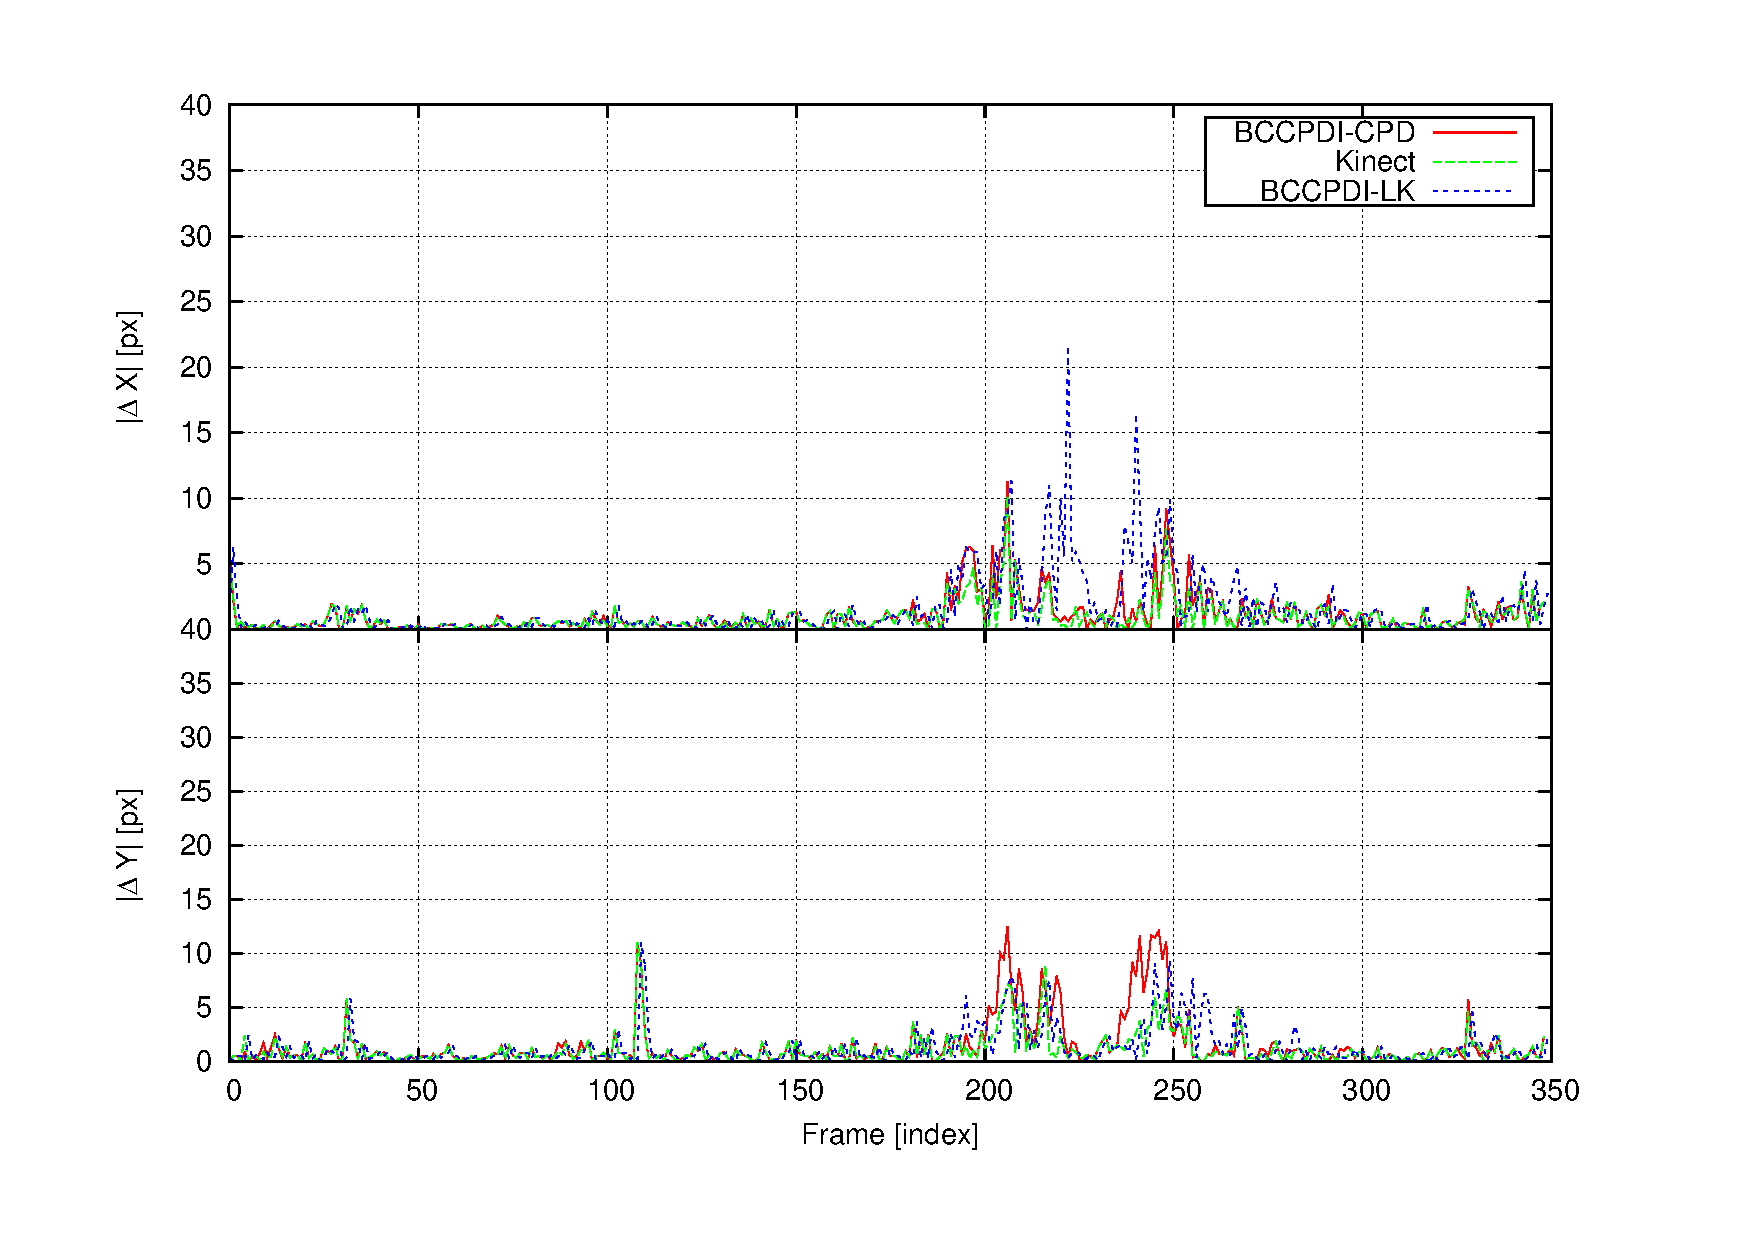
\includegraphics[width=\textwidth, trim=50 40 80 40,clip]{fig29.pdf}
%                 \caption*{Left knee}
%         \end{subfigure}%        
  \end{figure}
  \end{center}
\end{frame}

\begin{frame}[plain]{Final algorithm evaluation}
 \begin{figure}
  \includemovie[autoplay, repeat, controls]{\textwidth}{0.8\textheight}{/home/nestor/Seafile/Videos/Tesis/cp02/contour_flow_eval.mp4}
 \end{figure}
\end{frame}

\subsection{Evaluation of Stereo 3D Reconstruction Algorithms}

\begin{frame}{Algorithms}
  Three dense reconstruction algorithms tested:
  \begin{itemize}
   \item Census Cost Semi-Global Matching (Census-SGM) \footnote{\cite{Hirschmuller2005, Hirschmuller2009}}
   \item Birchfield-Tomasi Semi-Global Matching (BT-SGM)\footnote{\cite{Hirschmuller2005, Birchfield1998}, \url{http://opencv.org}}
   \item Efficient Large-Scale Stereo Matching (ELAS) \footnote{\cite{Geiger2011}}
  \end{itemize}


  \note {
    \begin{itemize}
     \item LIDAR-based GT takes time to be produced and FC is an indirect measurement.
     \item The use of a third camera allows to directly compare a reconstructed view with the actual images w/o manual intervention.

     \item NCC is calculated as described by Morales et al.

     \item It is suggested a configuration of 20 cm btween ref and match, and the ctrol camera is at 50 cm from ref camera
     \item In our conf, it is 24 and 12, respectively, as we use a precalibrated trinocular camera.
    \end{itemize}
  }
\end{frame}

% \begin{frame}{Algorithms}
%   \framesubtitle{Semi-Global Matching}
%   
%   \begin{itemize}
%     \item Disparity search range is reduced
%     \begin{itemize}
%       \item A set of sparse, robustly matched control points is found.
%       \item A 2D mesh is generated via Delaunay triangulation.
%       \item A prior is created from this mesh
%     \end{itemize}
%   \end{itemize}
% 
%   \note {
%     By computing a piecewise linear function induced by the support point disparities and the triangulated mesh.
%   }
% \end{frame}
% 
% \begin{frame}{Algorithms}
%   \framesubtitle{Efficient Large-Scale Stereo Matching (ELAS)}
%   
%   \begin{itemize}
%     \item Gets the disparity map D by minimizing \\
%     \begin{center} $E(D) = E_{data}(D) + E_{smooth}(D)$ \end{center}
%     \item NP-complete (but tractable using DP).
%     \item Two cost metrics:
%     \begin{enumerate}
%       \item Census cost metric.
%       \begin{itemize}
% 	\item Hamming distance of the Census transform of a 5x5 window.
%       \end{itemize}
%       \item  Birchfield-Tomasi cost metric.
%     \end{enumerate}
%   \end{itemize}
% 
%   \note {
%     \begin{itemize}
%      \item $E_{data}$ is the pixel-wise matching cost
%      \begin{itemize}
%       \item Sum of all pixels matching costs for the disparities of D
%      \end{itemize}
%      \item $E_{smooth}$ is the smooth constraint.
%      \begin{itemize}
%       \item adds a small penalty P1 to all px in the neighborhood of a pixel p for which the disparity varies by one
%       \item adds a higher penalty P2 if greater
%      \end{itemize}
%      \item SGM is no tractable in real time, unless we use a DP strategy
%      \item each pixel is used as the px-wise matching function, instead of the mutual information, as used in the original implementation.
%      \item Similar results, but reduces the overall processing burden
%      \item Each position C(p, d) of the cost volume is initialized with the number of differing bits btween the corresponding transformed values of left-right images.
%      \item We have used the freely available OpenCV implementation that uses BT pixel dissimilarity as cost metric to initialize the cost
%     \end{itemize}
%   }
% \end{frame}

\begin{frame}{Algorithms}
\begin{table}[h!]
\begin{center}
\resizebox{\columnwidth}{!} {
\begin{tabular}{|l|c|c|c|c|c|}
 \cline{2-6}
 \multicolumn{1}{ c|}{} & \multicolumn{3}{ c| }{Census-SGM} &
 \multicolumn{1}{ c| }{\multirow{2}{*}{BT-SGM}} &
 \multicolumn{1}{ c| }{\multirow{2}{*}{ELAS}} \\ \cline{2-4}
 \multicolumn{1}{c|}{} & Config 1 & Config 2 & Config 3 & & \\ \cline{2-6}
 \hline \hline
 Gaussian filter & $\surd$ & $\surd$ & $\surd$ & - & - \\
 Sparse Census mask & - & - & - & - & - \\
 Ternarized Census & - & - & - & - & - \\
 Hamming scores aggregation  & - & - & - & - & - \\
 Uniqueness constraint & 10 & 20 & 20 & 10 & 15 \\
 Adaptive mean & $\surd$ & $\surd$ & $\surd$ & - & $\surd$ \\
 Despeckle filter & $\surd$ & $\surd$ & $\surd$ & $\surd$ & $\surd$ \\
 Gap filter & $\surd$ & $\surd$ & - & - & $\surd$ \\
 \hline \hline
 Other parameters & \multicolumn{3}{ |c }{$P_1=10$, $P_2=50$, L/R check} &
 \multicolumn{1}{ |c }{see \footnote{\url{http://www.cvlibs.net/datasets/kitti/eval\_stereo\_flow.php}}} &
 \multicolumn{1}{ |c| }{see \footnotemark[\value{footnote}]} \\
 \hline
\end{tabular}
}
\end{center}
\end{table}
\end{frame}

% \begin{frame}{Results}
%   \includegraphics<1>{algo_bpp_ee3}
%   \includegraphics<2>{algo_avg_ee3}
%   \includegraphics<3>{algo_dens_ee3}
%   \includegraphics<4>{algo_nfc_perc}
%   \includegraphics<5>{algo_ncc}
%   
%   \note{
%   \begin{itemize}
%     \item We have selected conf. 2 as the best compromise btween reconstruction quality and map density
%     \item A comparison w/ the other 2 approaches is shown
%     \item At 90th percentile  the bad px percentage is cut around 7.5\% w.r.t. The baseline conf
%     \item By about 4.5\% if compared to BT-SGM
%     \item Avg error is reduced ny 0.15 px w/ Census-SGM conf 2, as well as w/ ELAS
%     \item Missing px increases to around 35\% (12\% more than baseline)
%     \item However, a substantial portion of the additional unreconstructed points is due to the improved error suppression capabilities of the algorithm.
%     \item NFC evaluation produces results which are in line w/ the one obtained with the LGT test
%     \item Census-SGM conf 2 is measurably and consistently better than the alternative approaches (winning algorithm in this comparison)
%     \item NCC scores for the ELAS and BT-SGM are quite close, and better than the Census-SGM baseline configuration
%     \item The placement of Census-SGM conf 2 looks suspicious
%     \item Data coming from this test will have to undergo further investigation before it can be trusted as a reliable indicator of an algorithm's performance
%   \end{itemize}
% 
%   }
% \end{frame}

\subsection{Stixel World}

\begin{frame}{Evaluation method}
\begin{itemize}
    \item Four different evaluations:
    \begin{enumerate}
      \item Quality of the clustering
      \item Depth accuracy
      \item Tracking
      \item Computational time
    \end{enumerate}
    \item \emph{Bahnhoff} sequence\footnote{\cite{ess2009robust}}
    \begin{itemize}
	\item 7400 obstacle annotations with height $\geq 40\,px$
	\item 999 stereo pairs
	\item $640 \times 480$ pixels
	\item 15 fps
    \end{itemize}
\end{itemize}

\end{frame}

\begin{frame}[plain]{Clustering}
  \begin{center}
    \only<1> {
      \vspace{-0.5cm}
      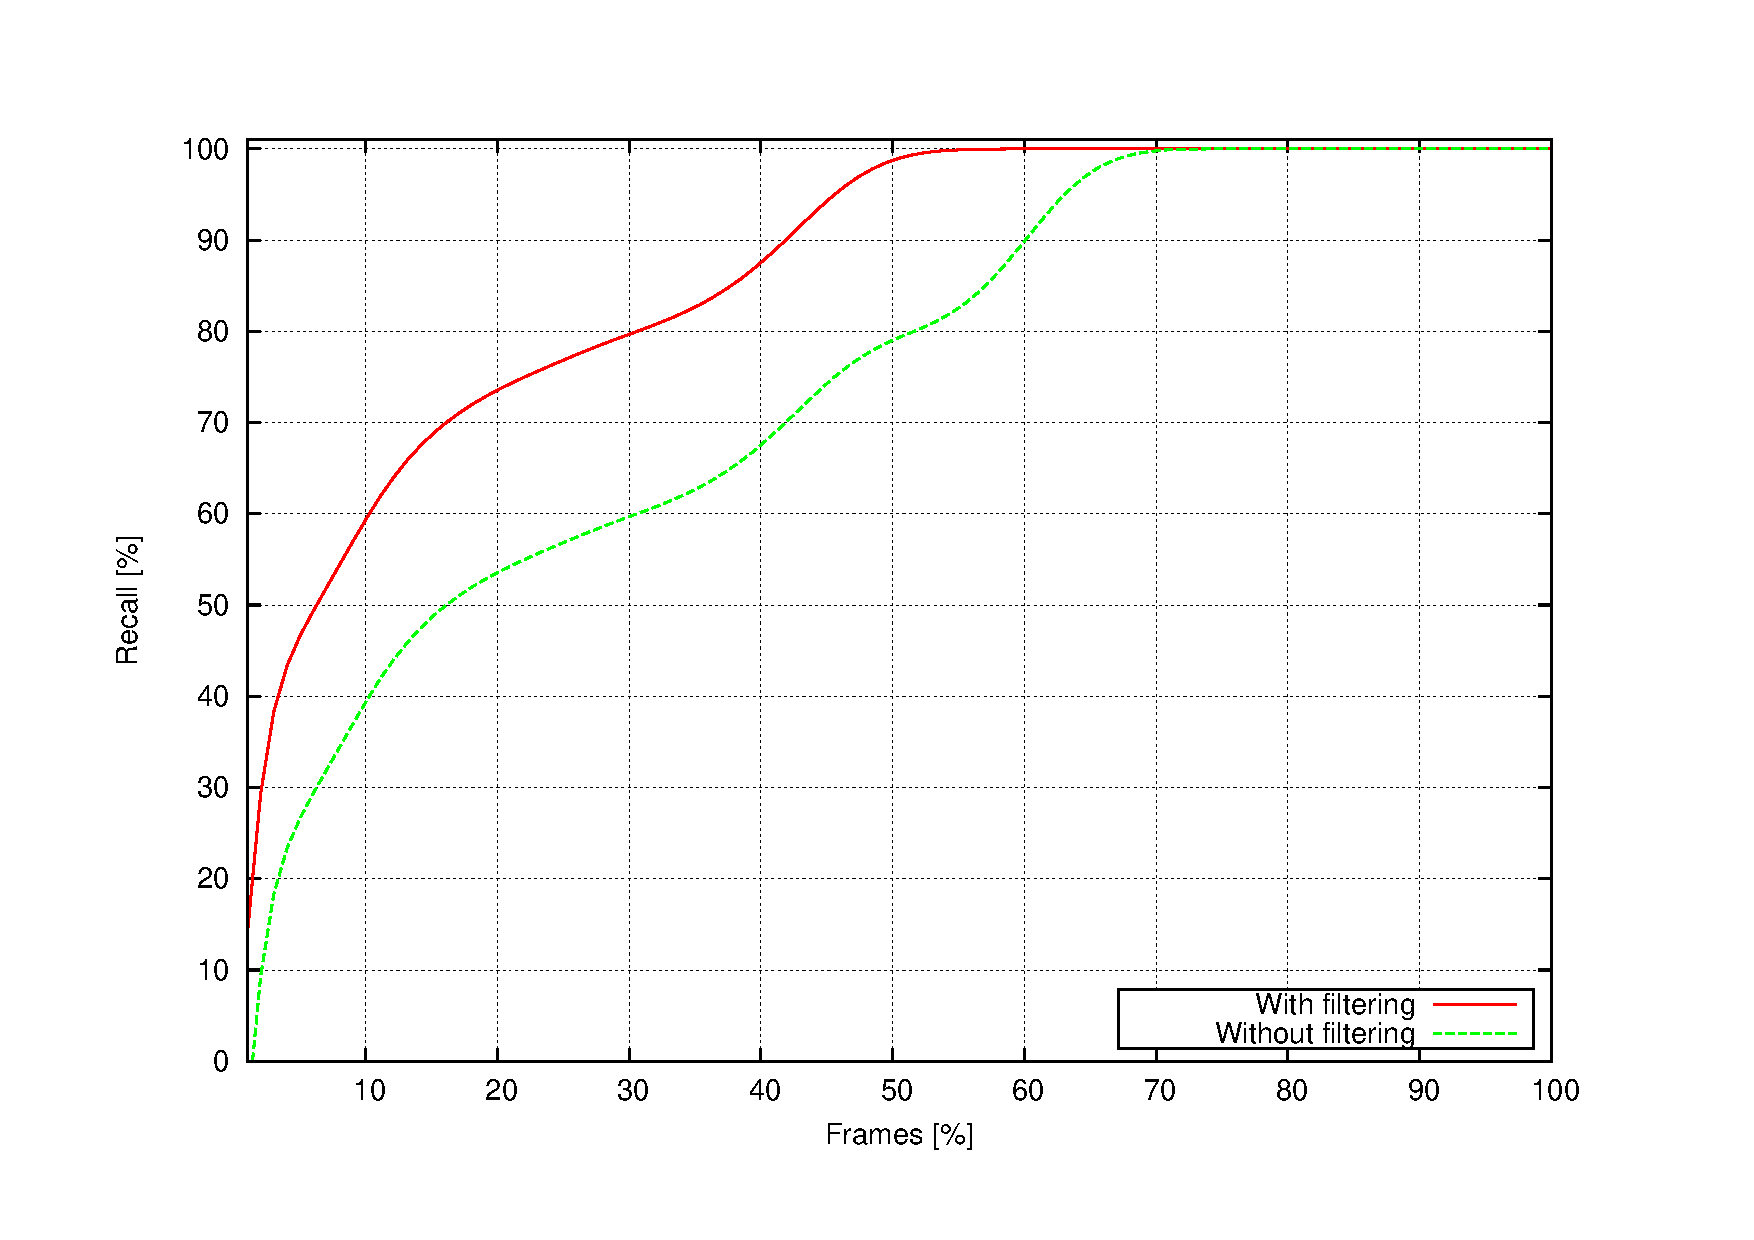
\includegraphics[height=1.1\textheight]{detectionRate}
    }
    \only<2> {
    \begin{figure}
      \begin{subfigure}[b]{0.5\columnwidth}
	\centering
	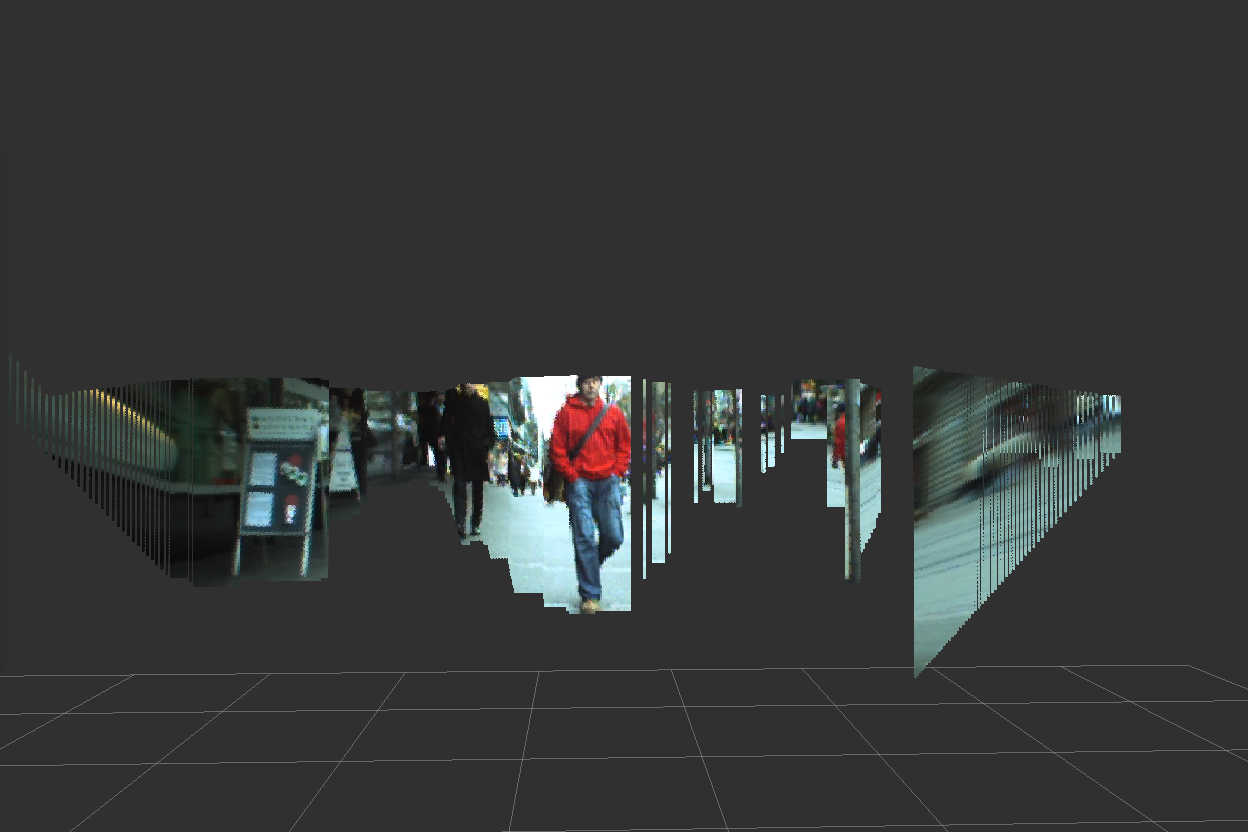
\includegraphics[width=\textwidth]{stixelsDetection}
	\caption*{\cite{benenson2012pedestrian}}
      \end{subfigure}%        
      ~
      \begin{subfigure}[b]{0.5\columnwidth}
	\centering
	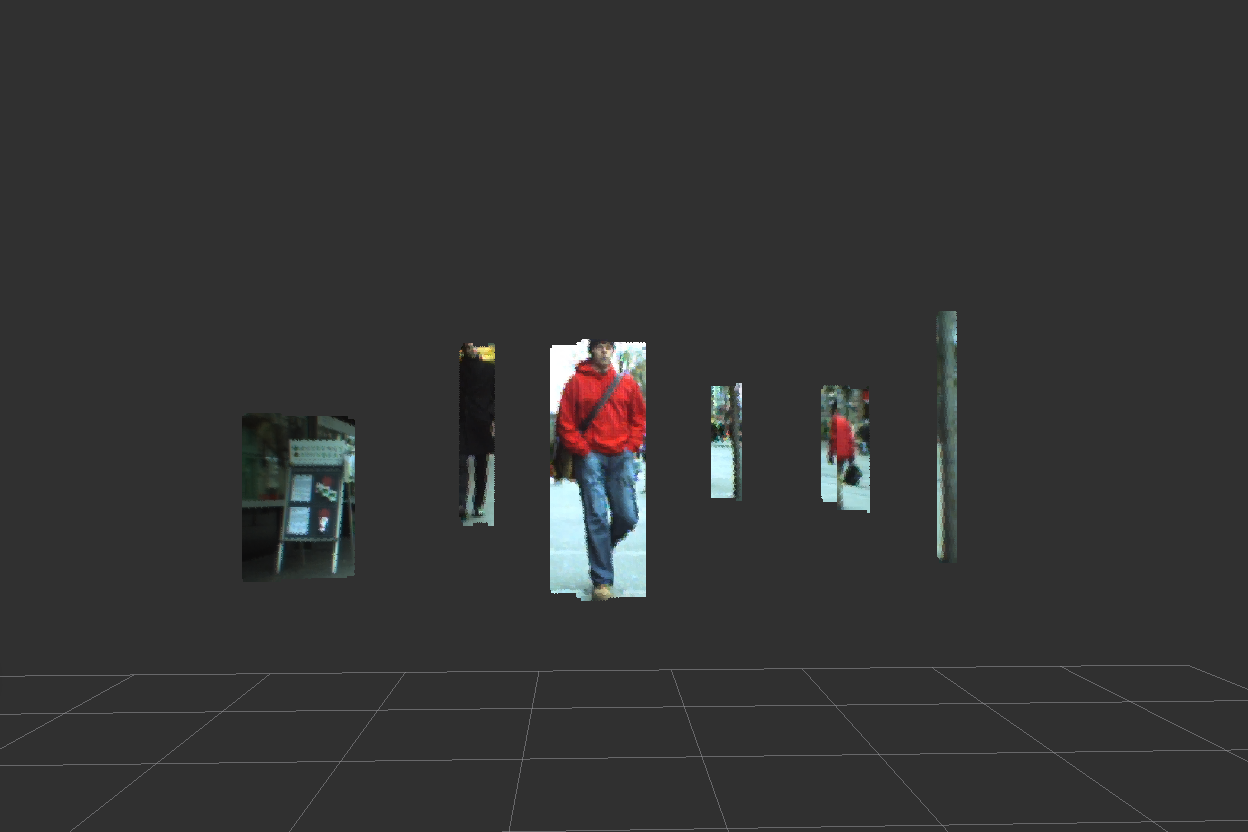
\includegraphics[width=\textwidth]{obstacleDetection}
	\caption*{Our method}
      \end{subfigure}%        
    \end{figure}
    }
  \end{center}
\end{frame}

\begin{frame}[plain]{Depth accuracy}
  \begin{center}
    \vskip-0.25cm
    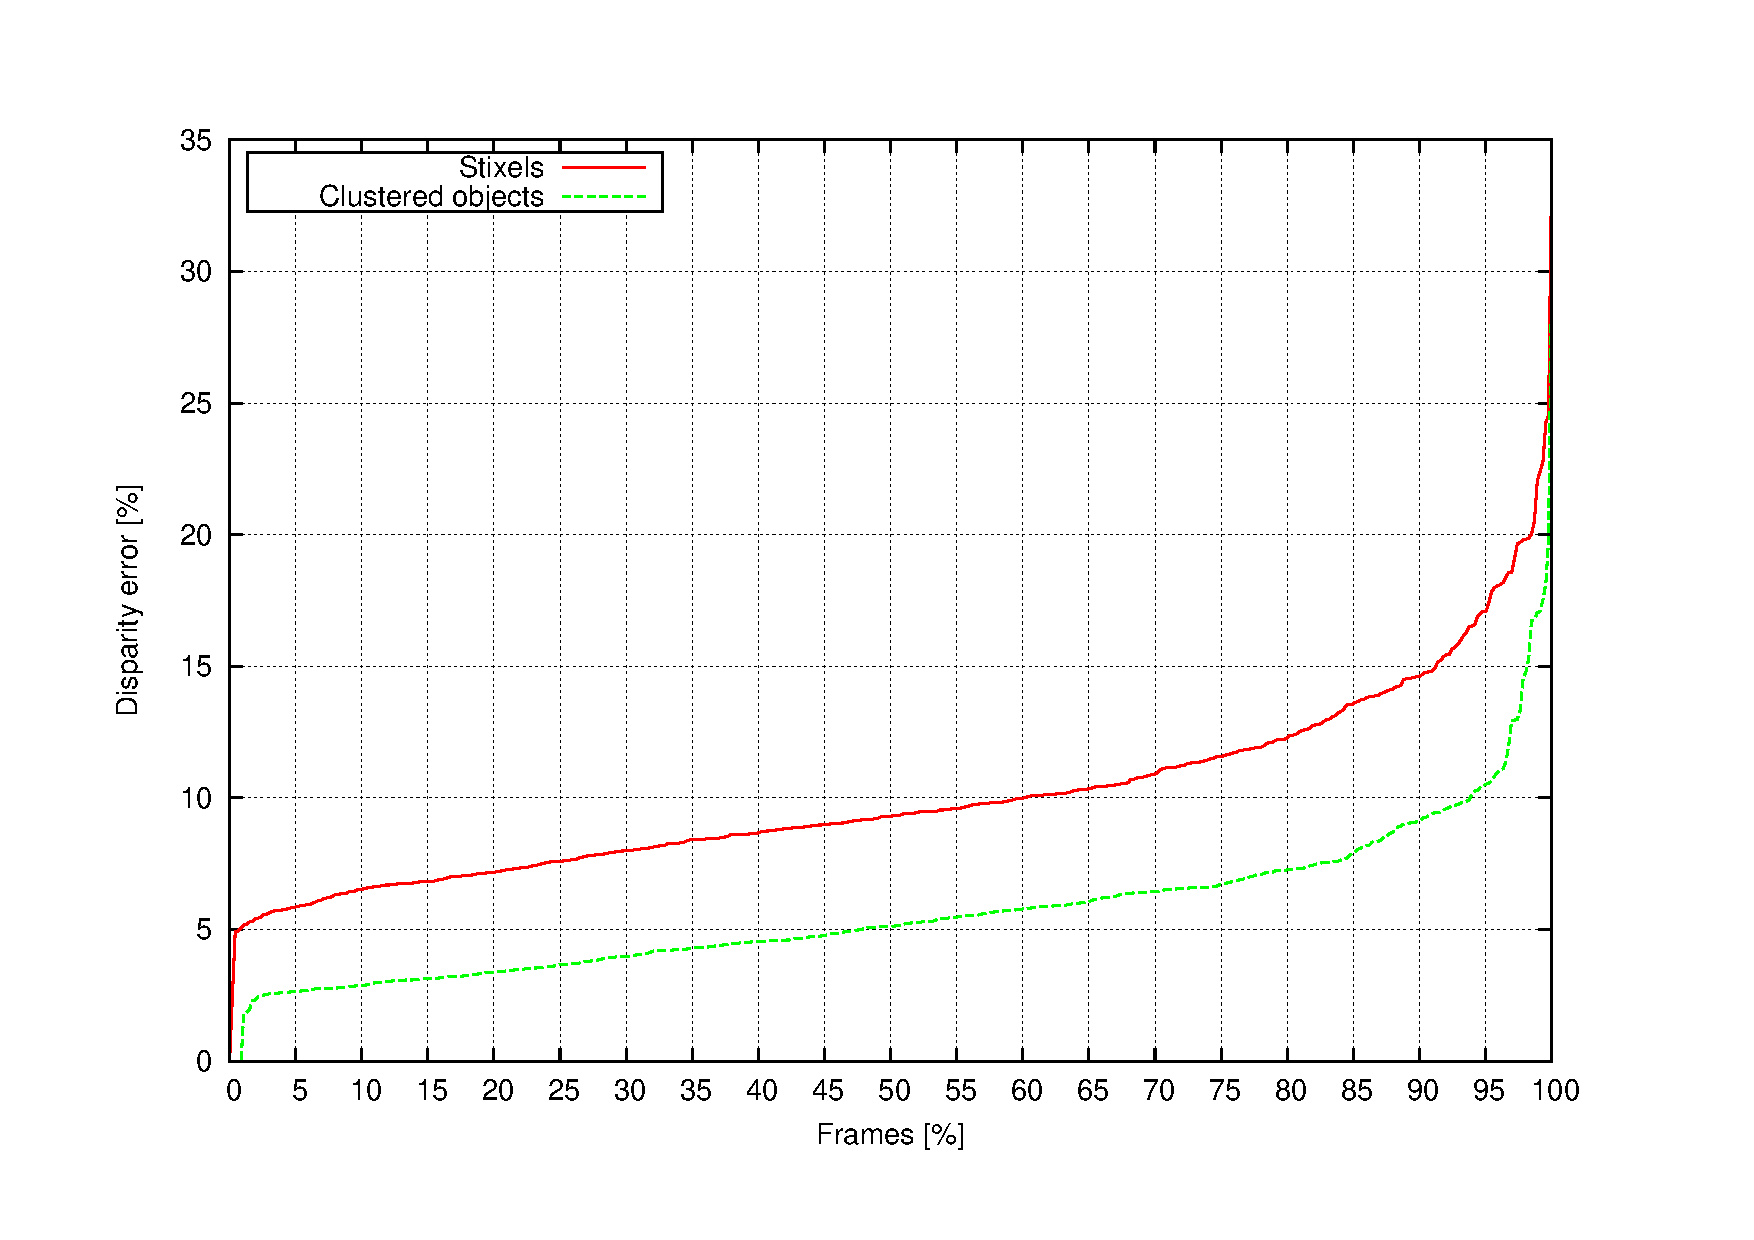
\includegraphics[width=\textwidth,height=0.55\textwidth,trim=50 40 80 60,clip]{disparity}
    \vskip-0.5cm
    \begin{figure}
	  \centering
	  \begin{subfigure}[b]{0.3\textwidth}
	      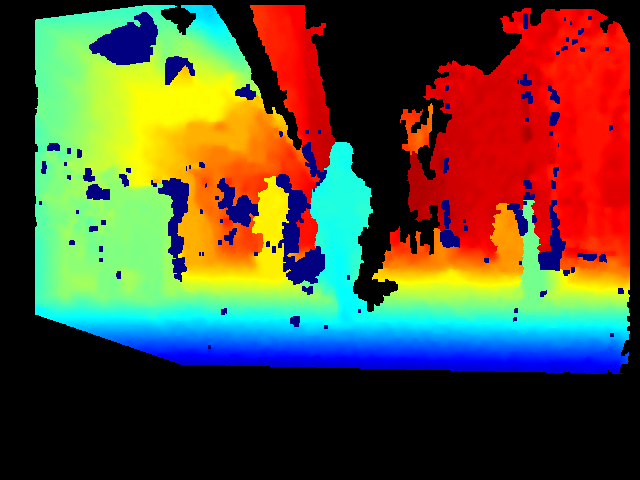
\includegraphics[height=0.3\figuresheight]{elas}
	  \end{subfigure}% 
	  \begin{subfigure}[b]{0.3\textwidth}
	      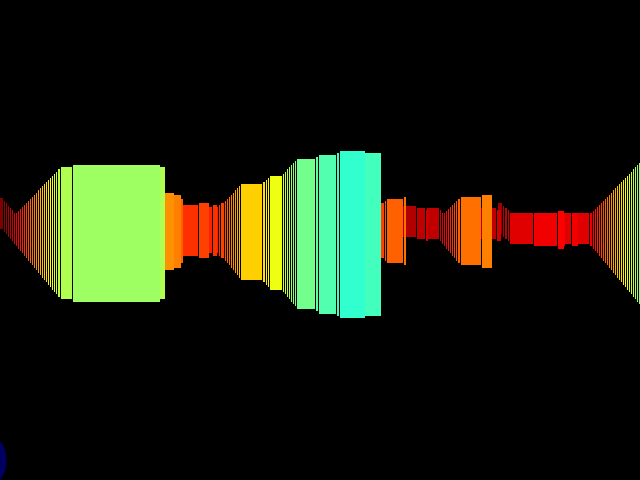
\includegraphics[height=0.3\figuresheight]{stixels}
	  \end{subfigure}%       
	  \begin{subfigure}[b]{0.3\textwidth}
	      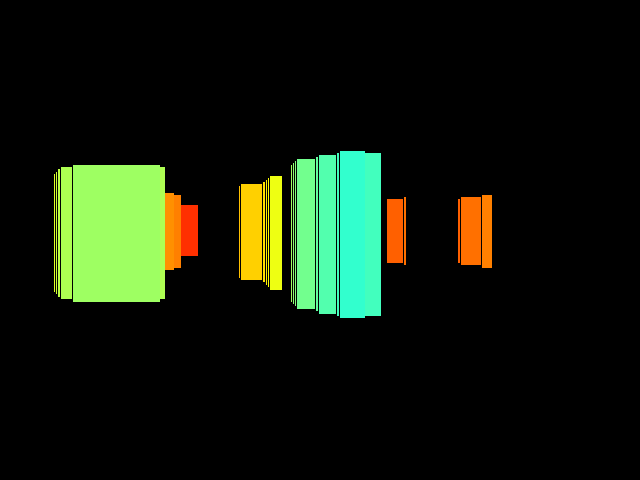
\includegraphics[height=0.3\figuresheight]{objects}
	  \end{subfigure}%    
	  \begin{subfigure}[b]{0.1\textwidth}
	      
\includegraphics[height=0.3\figuresheight]{colorscale_jet}
	  \end{subfigure}% 
    \end{figure}
  \end{center}
\end{frame}

\begin{frame}[plain]{Tracking}
  \begin{center}
    \only<1> {
    \begin{table}
      \begin{center}
      \begin{tabular}{|c|c|c|c|c|}
	\hline
      \multirow{2}{*}{Name} & \multicolumn{3}{ c| }{Cost factors} & \multirow{2}{*}{Tracking Method} \\ \cline{2-4}
      & $\alpha_{SAD}$ & $\alpha_{hist}$ & $\alpha_{height}$ &  \\
      \hline
      Conf. 1 & 1 & 0 & 0 & \cite{gunyel2012stixels} \\
      Conf. 2 & 0.5 & 0 & 0.5 & \cite{gunyel2012stixels} \\
      \hline
      Conf. 3 & 1 & 0 & 0 & Two-level tracking \\
      Conf. 4 & 0.5 & 0 & 0.5 & Two-level tracking \\
      Conf. 5 & 0 & 1 & 0 & Two-level tracking \\
      Conf. 6 & 0 & 0.5 & 0.5 & Two-level tracking \\
      \hline
      Conf. 7 & 0 & 0 & 0 & Object tracking \\
      \hline
      \end{tabular}
      \end{center}
    \end{table}
    }
    \only<2> {
      \begin{overlayarea}{\textwidth}{\textheight}
	\begin{center}
	  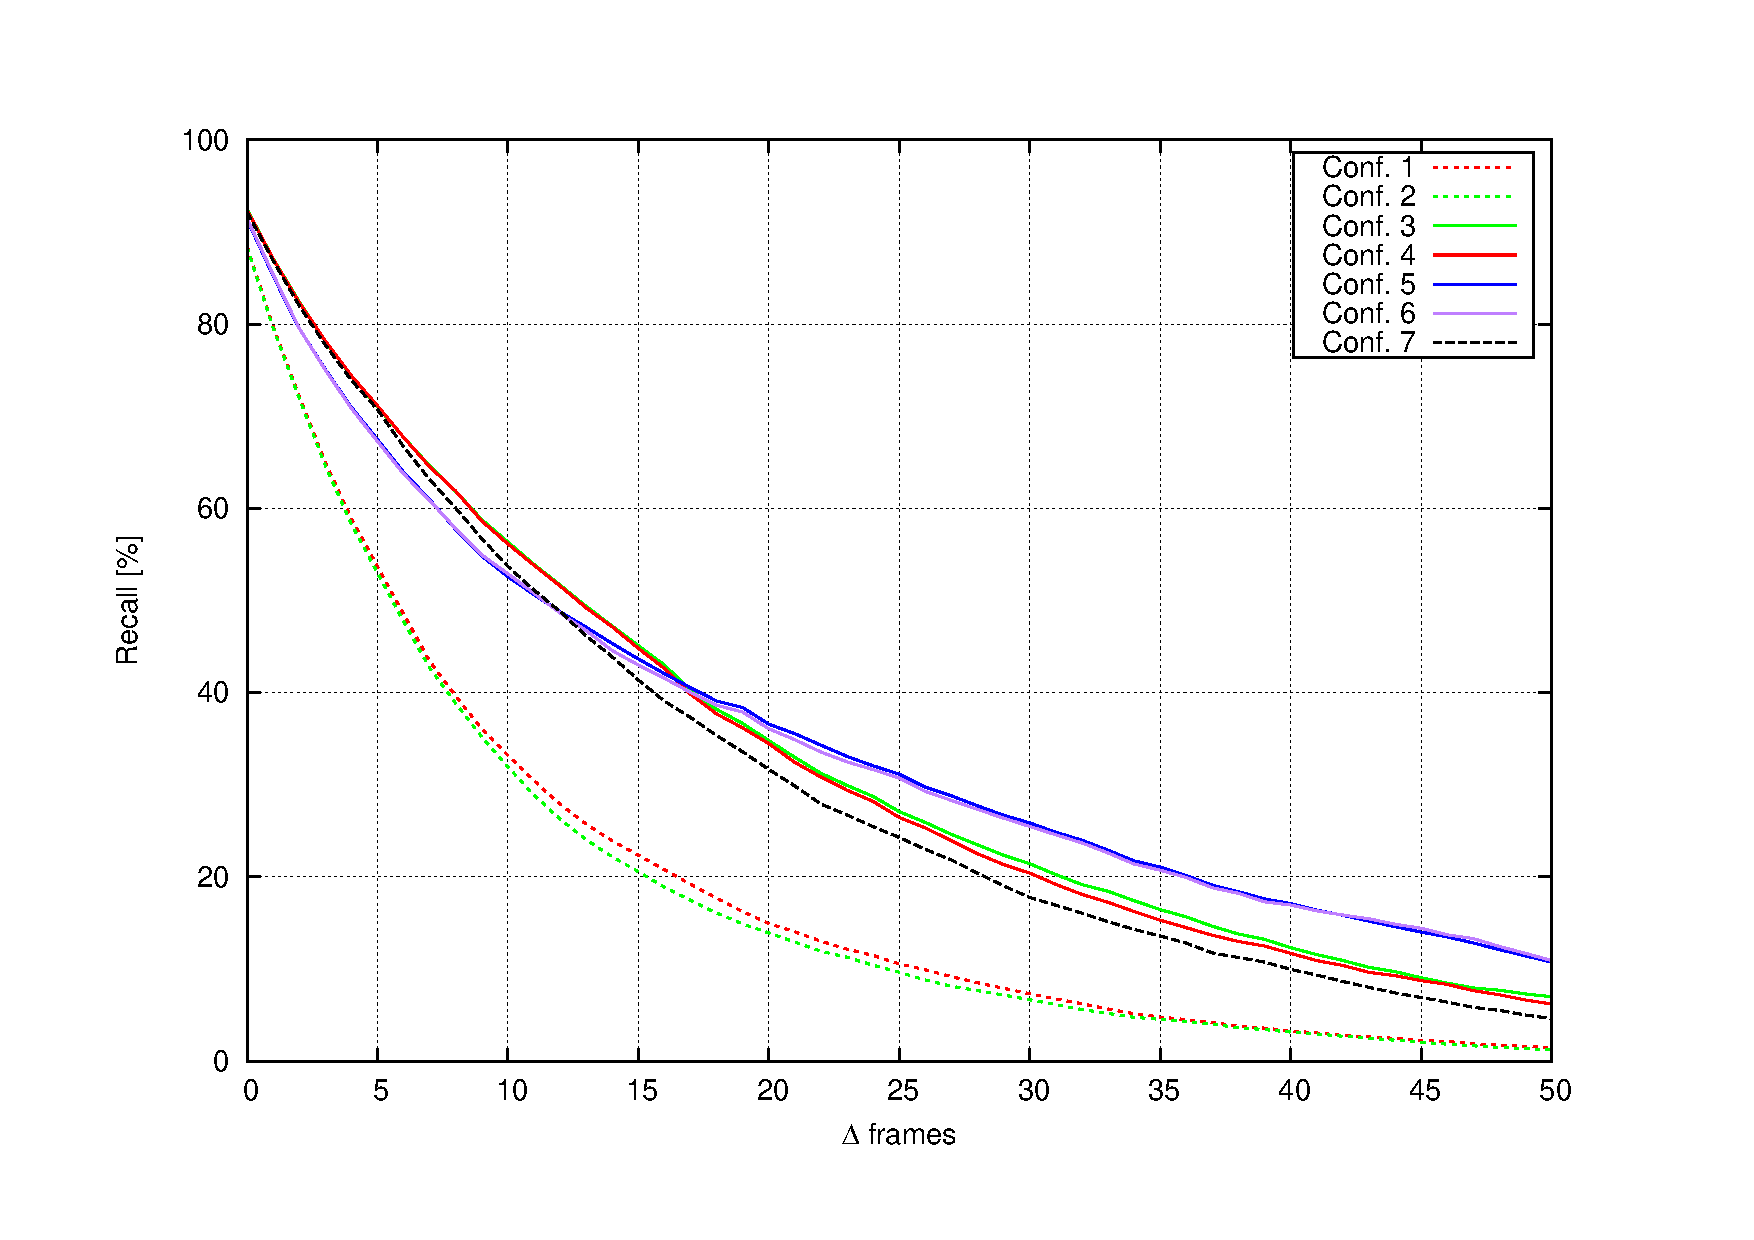
\includegraphics[height=1.1\textheight,trim=50 40 80 60,clip]{recall_vs_delta_frames}
	\end{center}
      \end{overlayarea}
      \begin{overlayarea}{\textwidth}{\textheight}
	\vspace{-8.25cm}
	\hspace{2.45cm}
	\begin{minipage}{0.6\textwidth}
	  \setbeamertemplate{blocks}[rounded][shadow=false]
	  \begin{block}{}
	    \tiny
	    \begin{table}
	      \begin{center}
	      \begin{tabular}{|c|c|c|c|c|}
		\hline
	      \multirow{2}{*}{Name} & \multicolumn{3}{ c| }{Cost factors} & \multirow{2}{*}{Tracking Method} \\ \cline{2-4}
	      & $\alpha_{SAD}$ & $\alpha_{hist}$ & $\alpha_{height}$ &  \\
	      \hline
	      Conf. 1 & 1 & 0 & 0 & \cite{gunyel2012stixels} \\
	      Conf. 2 & 0.5 & 0 & 0.5 & \cite{gunyel2012stixels} \\
	      \hline
	      Conf. 3 & 1 & 0 & 0 & Two-level tracking \\
	      Conf. 4 & 0.5 & 0 & 0.5 & Two-level tracking \\
	      Conf. 5 & 0 & 1 & 0 & Two-level tracking \\
	      Conf. 6 & 0 & 0.5 & 0.5 & Two-level tracking \\
	      \hline
	      Conf. 7 & 0 & 0 & 0 & Object tracking \\
	      \hline
	      \end{tabular}
	      \end{center}
	    \end{table}
	  \end{block}
	\end{minipage}
      \end{overlayarea}
    }
    \only<3> {
      \begin{figure}
        \centering
        \begin{subfigure}[b]{0.45\textwidth}
	  \begin{tabular}{c}
	    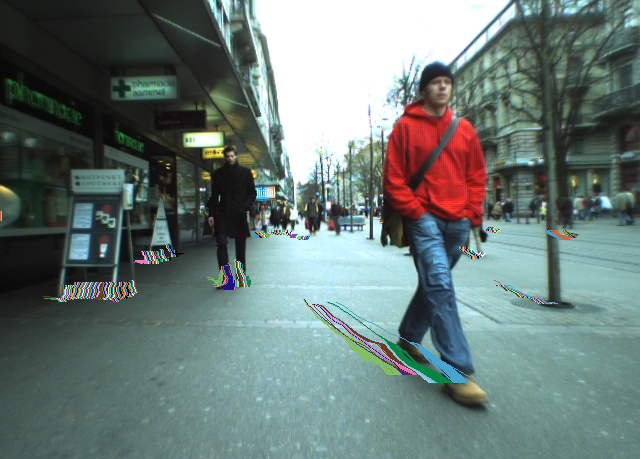
\includegraphics[width=\textwidth]{trackingConf1}
	  \end{tabular}
	  \caption*{Conf. 1}
        \end{subfigure}% 
        ~
        \begin{subfigure}[b]{0.45\textwidth}
	  \begin{tabular}{c}
	    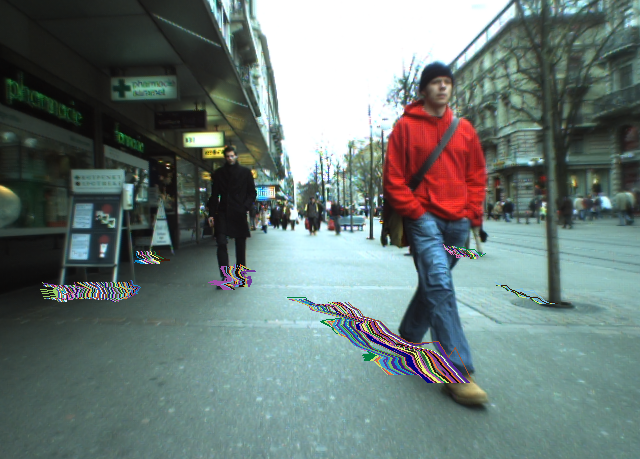
\includegraphics[width=\textwidth]{trackingConf5}
	  \end{tabular}
	  \caption*{Conf. 5}
        \end{subfigure}%       
        
        \begin{subfigure}[b]{0.45\textwidth}
	  \begin{tabular}{c}
	    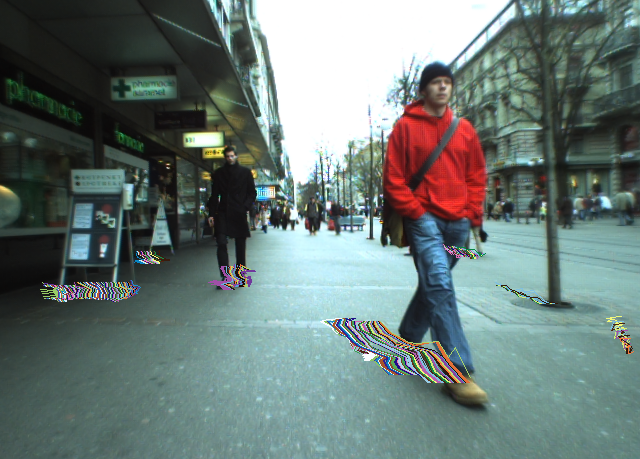
\includegraphics[width=\textwidth]{trackingConf7}
	  \end{tabular}
	  \caption*{Conf. 7}
        \end{subfigure}%
      \end{figure}
    }
    \only<4> {
      \begin{overlayarea}{\textwidth}{\textheight}
	\begin{center}
	  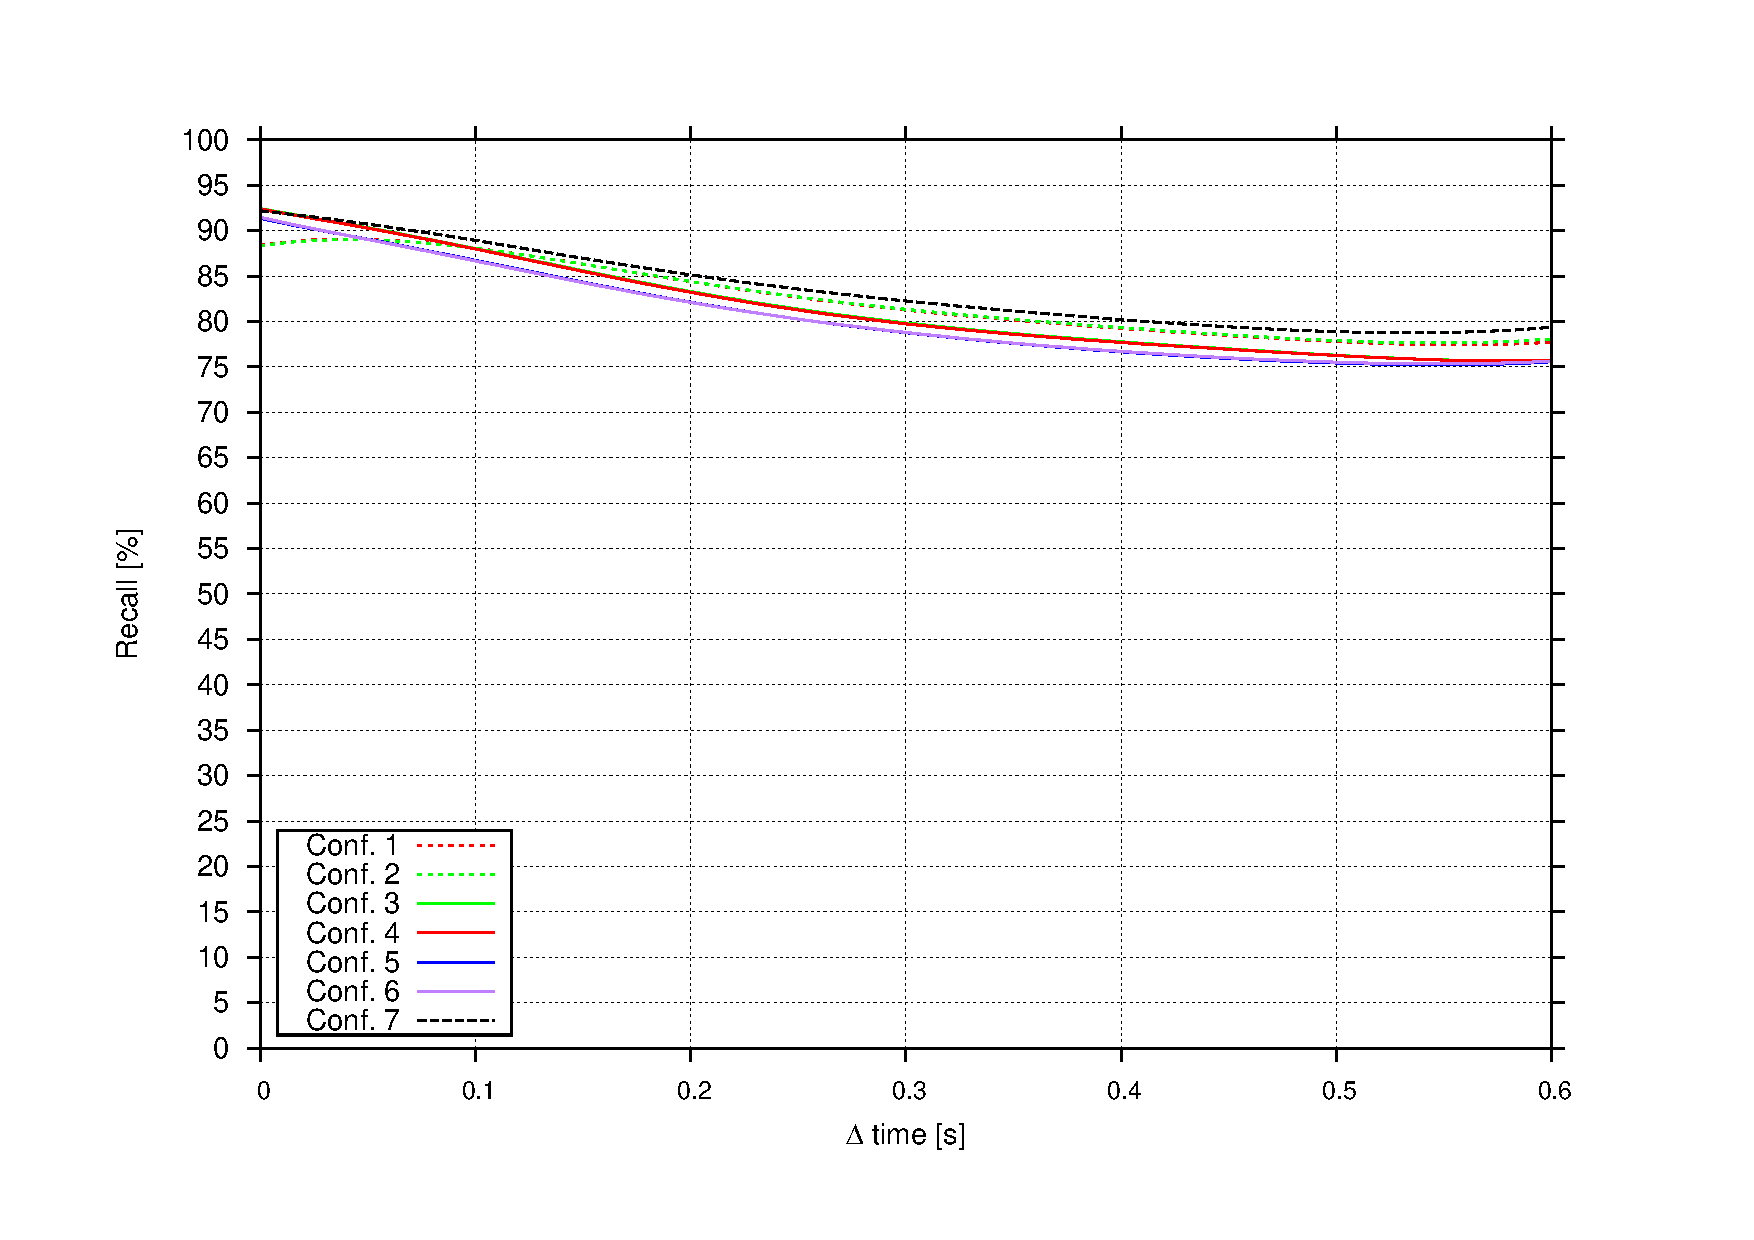
\includegraphics[height=1.1\textheight,trim=50 40 80 60,clip]{recall_vs_step}
	\end{center}
      \end{overlayarea}
      \begin{overlayarea}{\textwidth}{\textheight}
	\vspace{-3.5cm}
	\hspace{4.0cm}
	\begin{minipage}{0.6\textwidth}
	  \setbeamertemplate{blocks}[rounded][shadow=false]
	  \begin{block}{}
	    \tiny
	    \begin{table}
	      \begin{center}
	      \begin{tabular}{|c|c|c|c|c|}
		\hline
	      \multirow{2}{*}{Name} & \multicolumn{3}{ c| }{Cost factors} & \multirow{2}{*}{Tracking Method} \\ \cline{2-4}
	      & $\alpha_{SAD}$ & $\alpha_{hist}$ & $\alpha_{height}$ &  \\
	      \hline
	      Conf. 1 & 1 & 0 & 0 & \cite{gunyel2012stixels} \\
	      Conf. 2 & 0.5 & 0 & 0.5 & \cite{gunyel2012stixels} \\
	      \hline
	      Conf. 3 & 1 & 0 & 0 & Two-level tracking \\
	      Conf. 4 & 0.5 & 0 & 0.5 & Two-level tracking \\
	      Conf. 5 & 0 & 1 & 0 & Two-level tracking \\
	      Conf. 6 & 0 & 0.5 & 0.5 & Two-level tracking \\
	      \hline
	      Conf. 7 & 0 & 0 & 0 & Object tracking \\
	      \hline
	      \end{tabular}
	      \end{center}
	    \end{table}
	  \end{block}
	\end{minipage}
      \end{overlayarea}
    }
  \end{center}
\end{frame}

\begin{frame}[plain]{Computational time}
  \begin{center}
    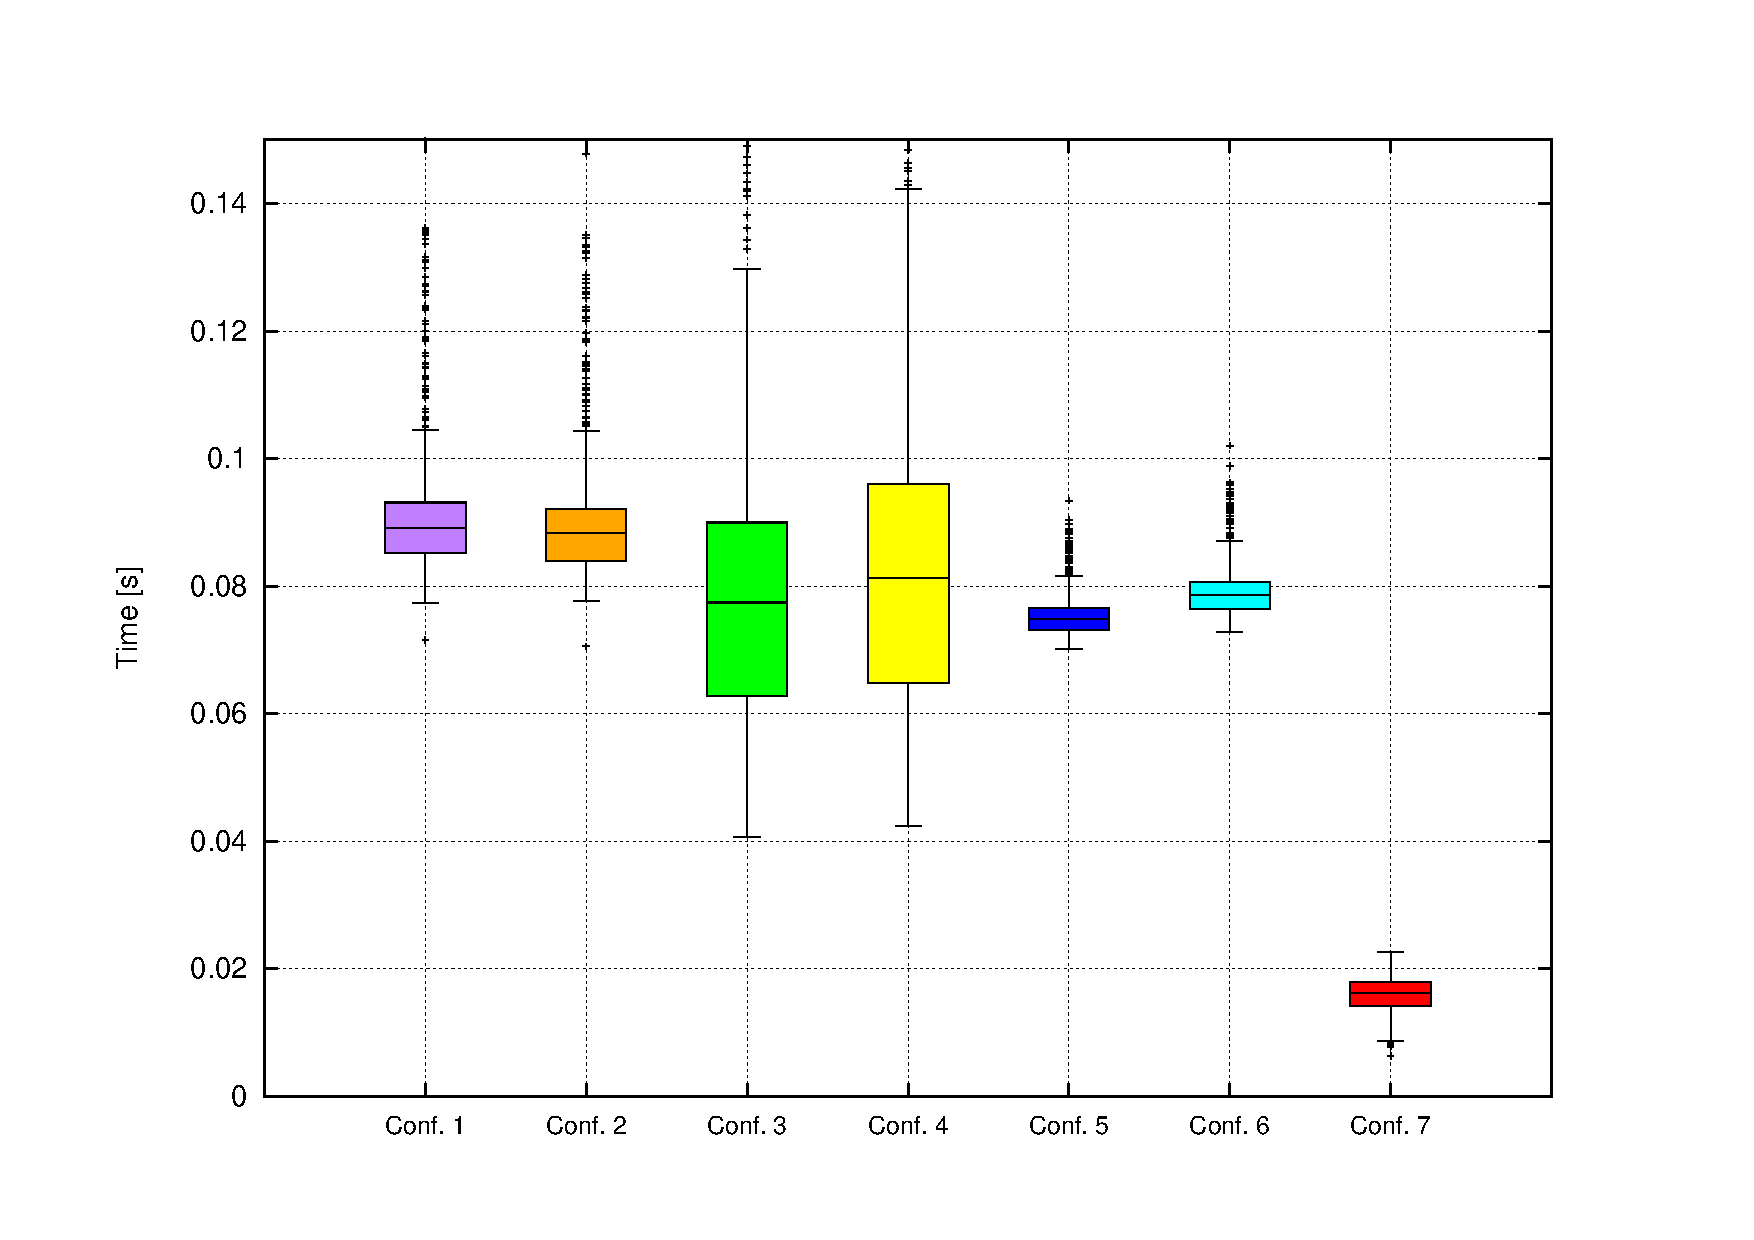
\includegraphics[height=0.8\textheight,trim=50 40 80 60,clip]{times_average}
    \tiny
    \begin{table}
      \begin{center}
	\begin{tabular}{|c|c|c|c|c|}
	  \hline
	\multirow{2}{*}{Name} & \multicolumn{3}{ c| }{Cost factors} & \multirow{2}{*}{Tracking Method} \\ \cline{2-4}
	& $\alpha_{SAD}$ & $\alpha_{hist}$ & $\alpha_{height}$ &  \\
	\hline
	Conf. 1 & 1 & 0 & 0 & \cite{gunyel2012stixels} \\
	Conf. 2 & 0.5 & 0 & 0.5 & \cite{gunyel2012stixels} \\
	\hline
	Conf. 3 & 1 & 0 & 0 & Two-level tracking \\
	Conf. 4 & 0.5 & 0 & 0.5 & Two-level tracking \\
	Conf. 5 & 0 & 1 & 0 & Two-level tracking \\
	Conf. 6 & 0 & 0.5 & 0.5 & Two-level tracking \\
	\hline
	Conf. 7 & 0 & 0 & 0 & Object tracking \\
	\hline
	\end{tabular}
      \end{center}
    \end{table}
  \end{center}
\end{frame}

\subsection{Particle Filter based Object Tracking}

\begin{frame}{Evaluation method}
  \begin{itemize}
   \item Four evaluation sets:
   \begin{enumerate}
    \item Input point cloud
    \item Ego-motion
    \item Detection
    \item Performance
   \end{enumerate}
   \item KITTI Vision Benchmark (Karlsruhe Institute of Technology)\footnote{\cite{geiger2013vision}}
  \end{itemize}
  \begin{center}
    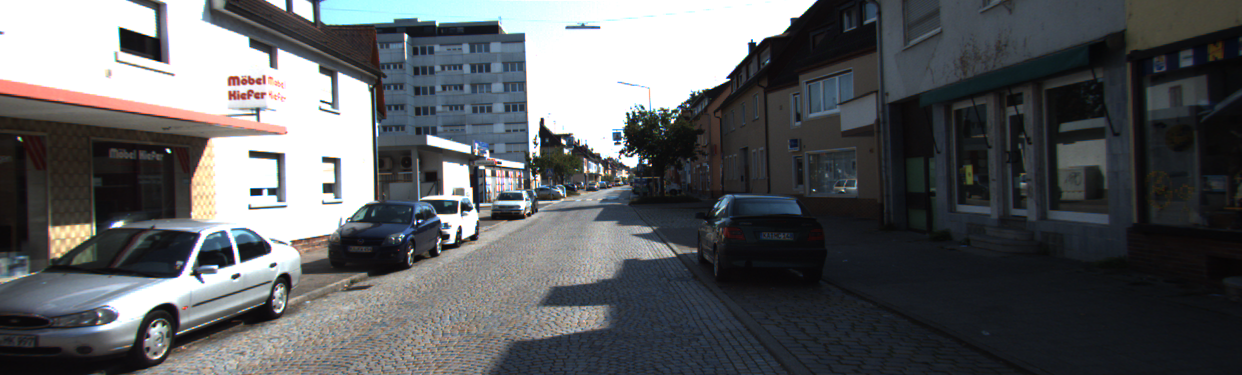
\includegraphics[height=0.4\textheight]{kitti}
  \end{center}
\end{frame}

\begin{frame}[plain]{Detection}
  \begin{center}
    \includegraphics<1>[height=1.1\textheight,trim=50 40 80 60,clip]{recall}
    \includegraphics<2>[height=1.1\textheight,trim=50 40 80 60,clip]{precision}
  \end{center}
\end{frame}

\begin{frame}[plain]{Performance}
  \begin{center}
    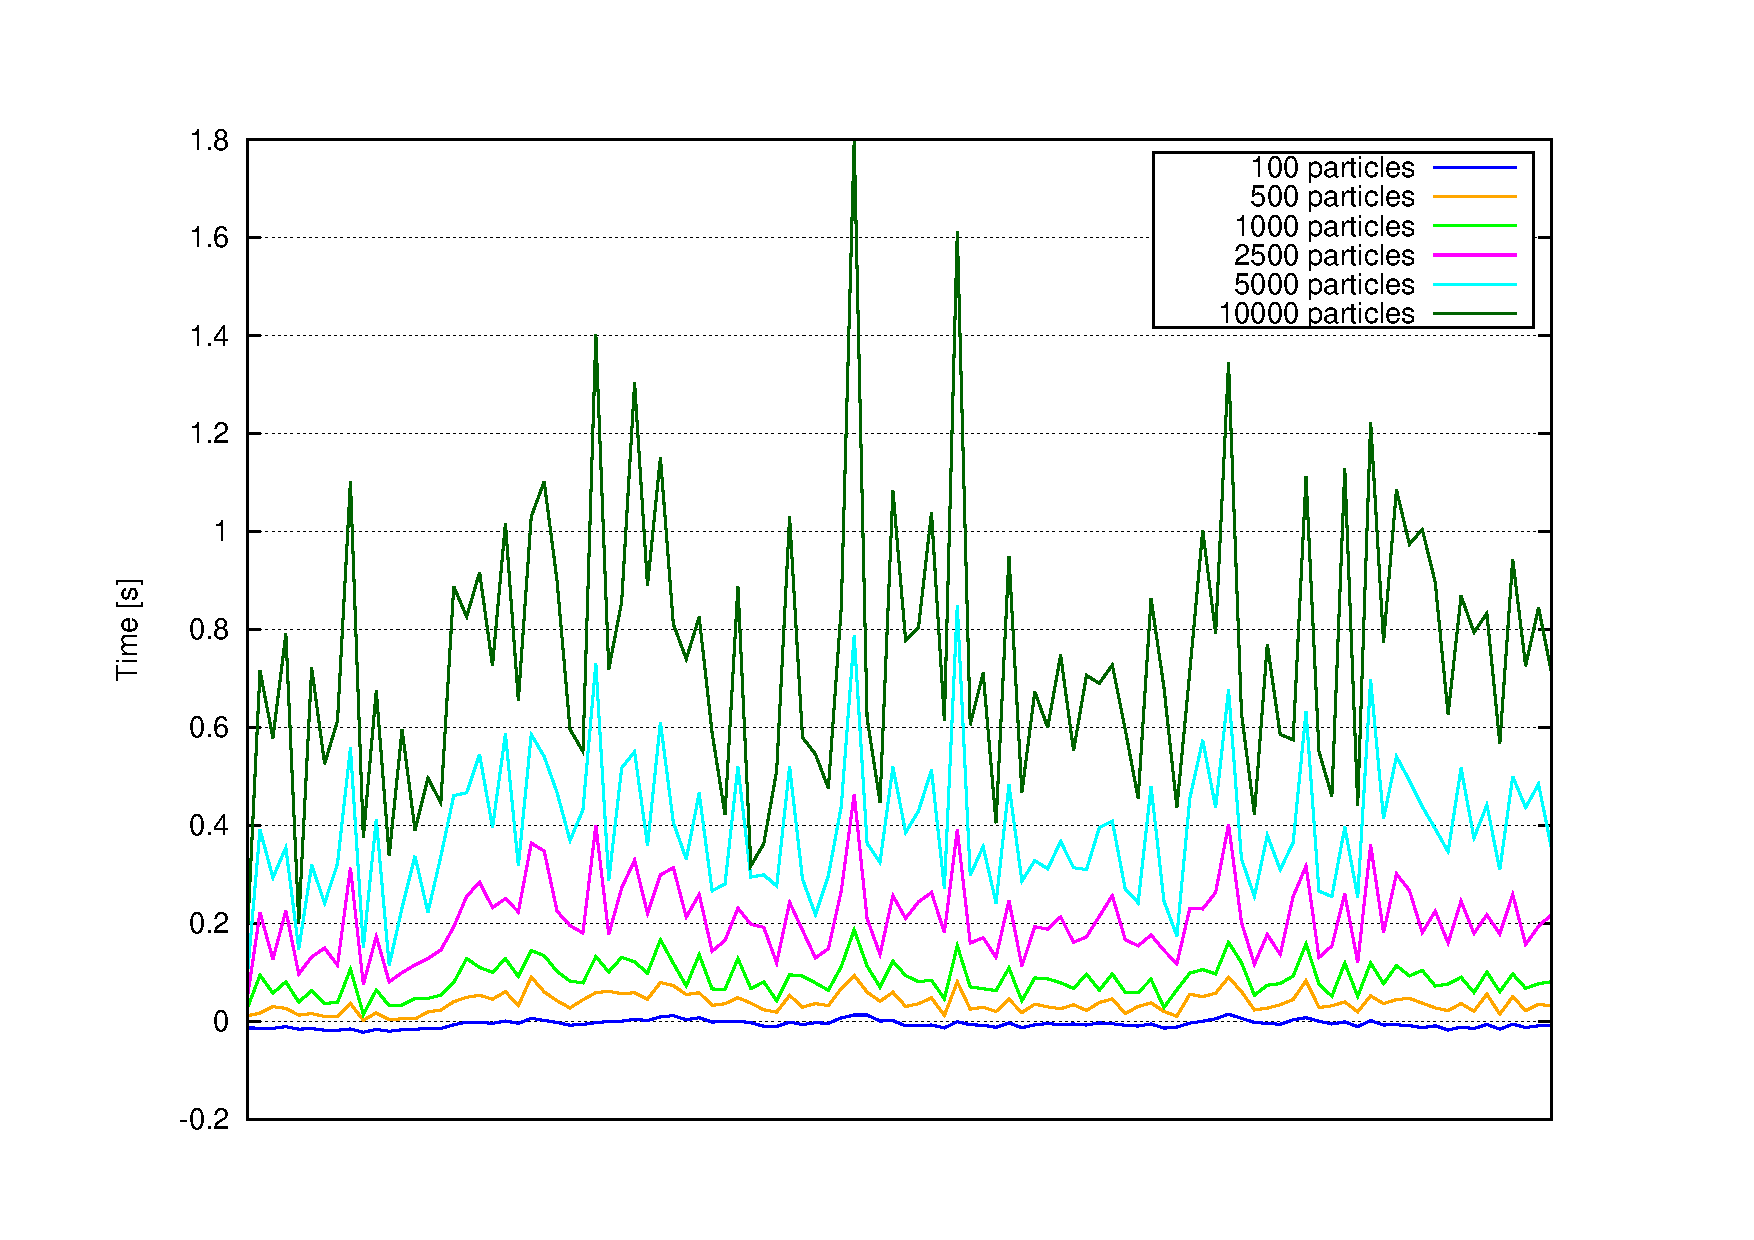
\includegraphics[height=1.1\textheight,trim=50 50 90 60, clip]{timesVsParticles}
  \end{center}
\end{frame}

\subsection{Global Planning}

\begin{frame}{Evaluation method}
  \begin{itemize}
    \item Comparison with other methods
    \begin{enumerate}
      \item Multiclass SVM (our method)
      \item Single SVM \citep{miura2006support}
      \item Voronoi
      \item Voronoi + SVM \citep{yang2012safe}
    \end{enumerate}
    \item Three metrics:
    \begin{enumerate}
      \item Average distance to obstacles
      \item Smoothness
      \item Length
    \end{enumerate}
  \end{itemize}
\end{frame}

% \begin{frame}{Average distance to obstacles}
%   \begin{center}
%     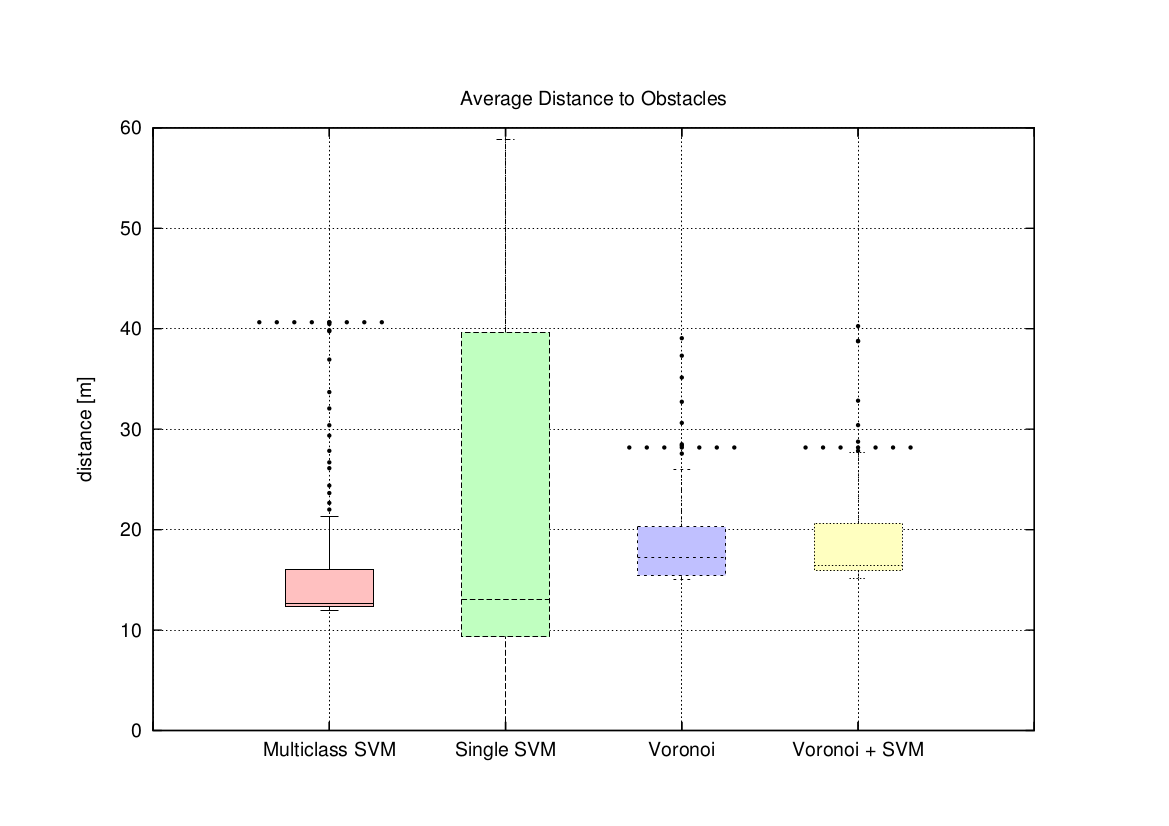
\includegraphics[width=0.8\textwidth,trim=55 50 85 60, clip]{figure11}
%   \end{center}
% \end{frame}
% 
% \begin{frame}{Smoothness}
%   \begin{center}
%     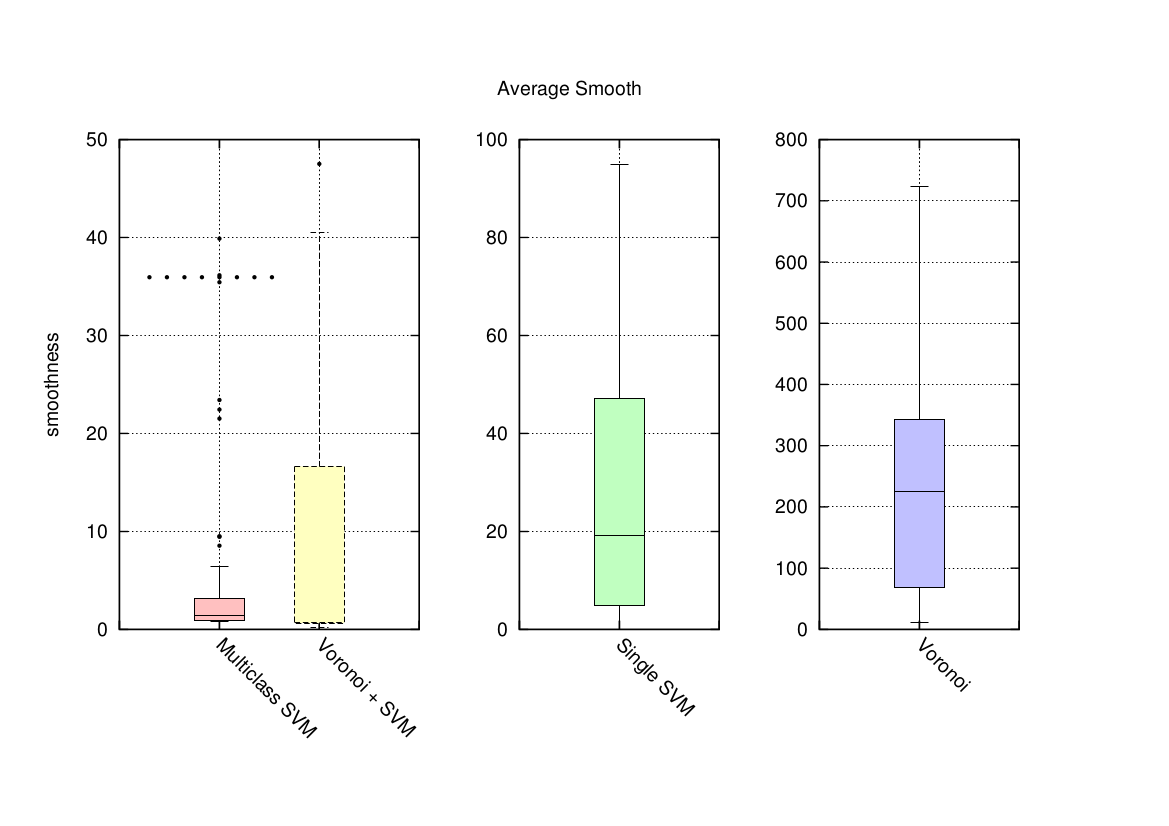
\includegraphics[width=0.8\textwidth,trim=55 50 85 60, clip]{figure12}
%   \end{center}
% \end{frame}
% 
% \begin{frame}{Length}
%   \begin{center}
%     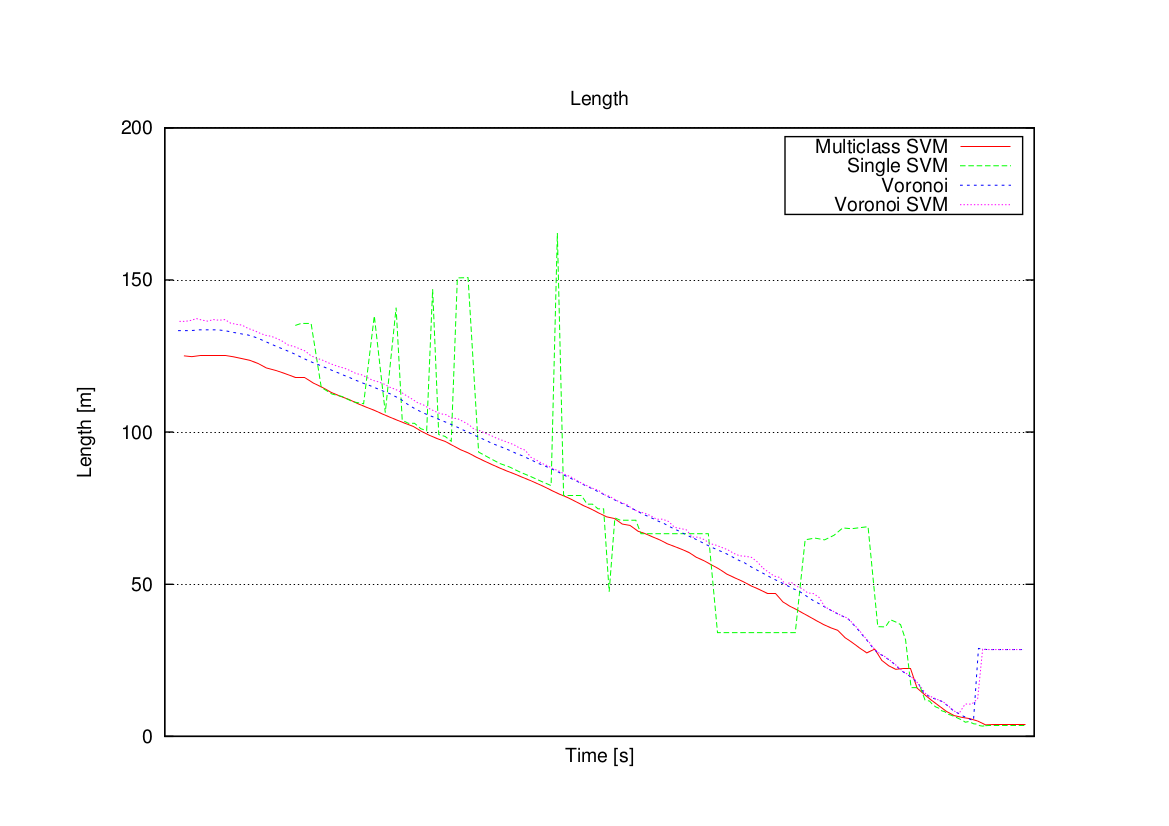
\includegraphics[width=0.8\textwidth,trim=55 45 85 60, clip]{figure13}
%   \end{center}
% \end{frame}

\begin{frame}[plain]{Global planning}
  \begin{center}
    \includemovie[autoplay, repeat, controls]{\linewidth}{.6\linewidth}{/home/nestor/Seafile/Videos/Tesis/cp06/four_methods.mp4}
  \end{center}
\end{frame}

\subsection{Local Planning}

\begin{frame}{Path following performance}
  \begin{center}
    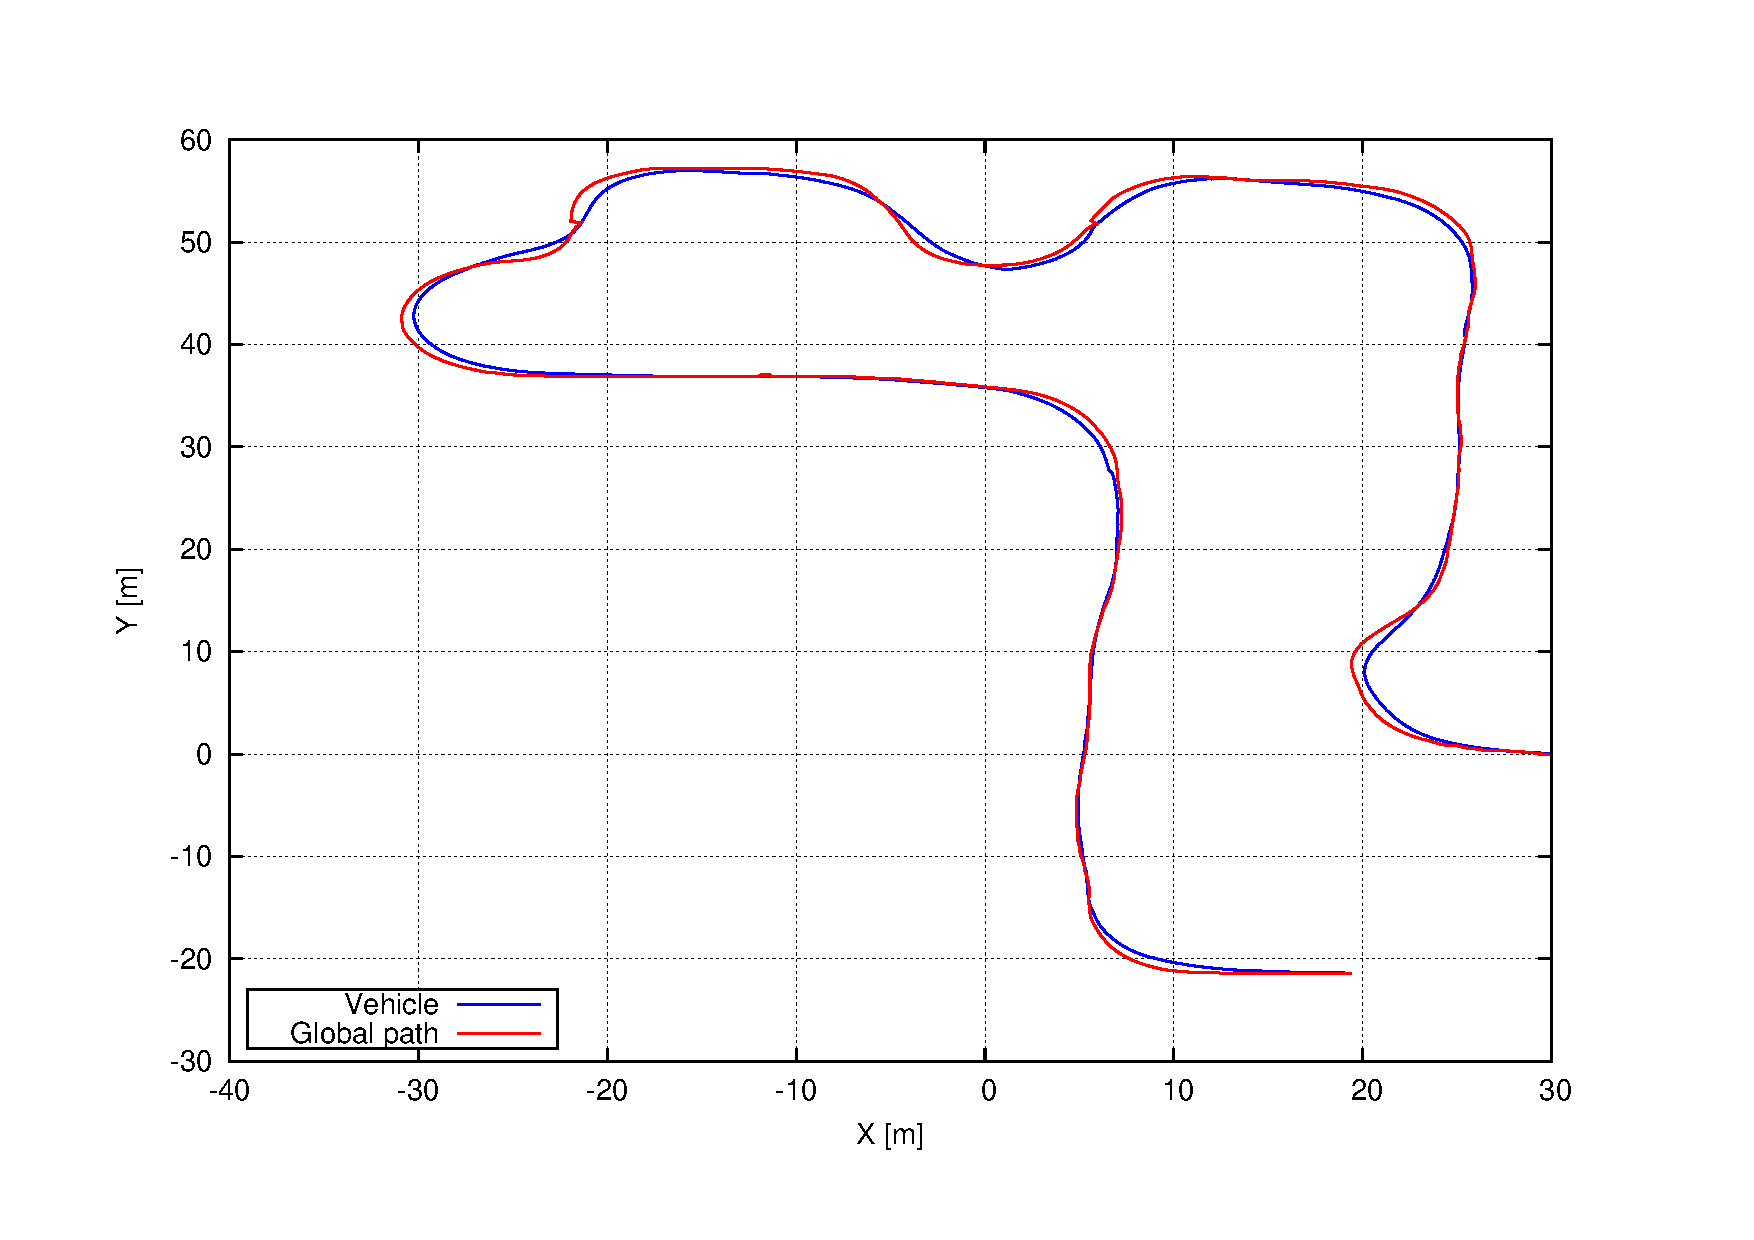
\includegraphics[height=0.8\textheight,trim=50 40 80 60, clip]{differences}
  \end{center}
\end{frame}

\begin{frame}[plain]{Costs}
  \begin{columns}
   \column[c]{0.5\textwidth}
    \begin{center}
      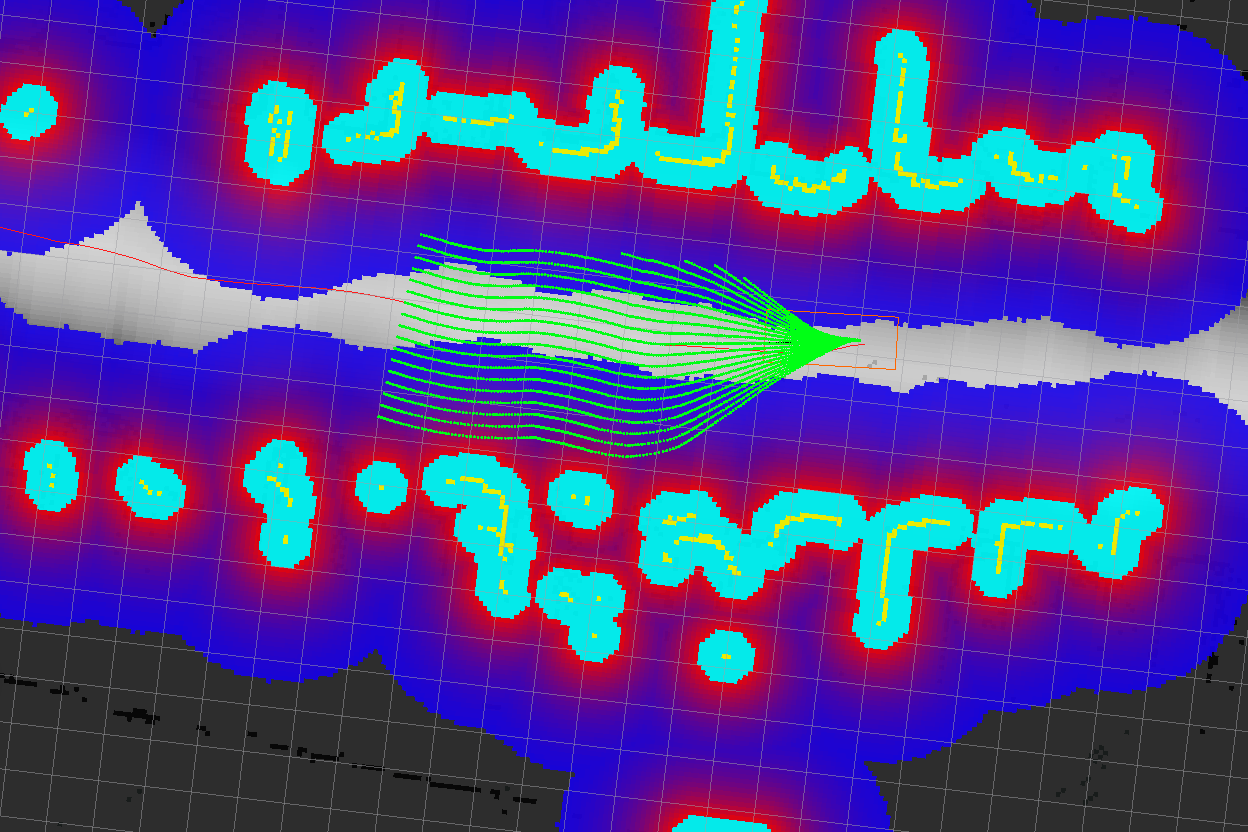
\includegraphics[width=\textwidth]{example4}\\
      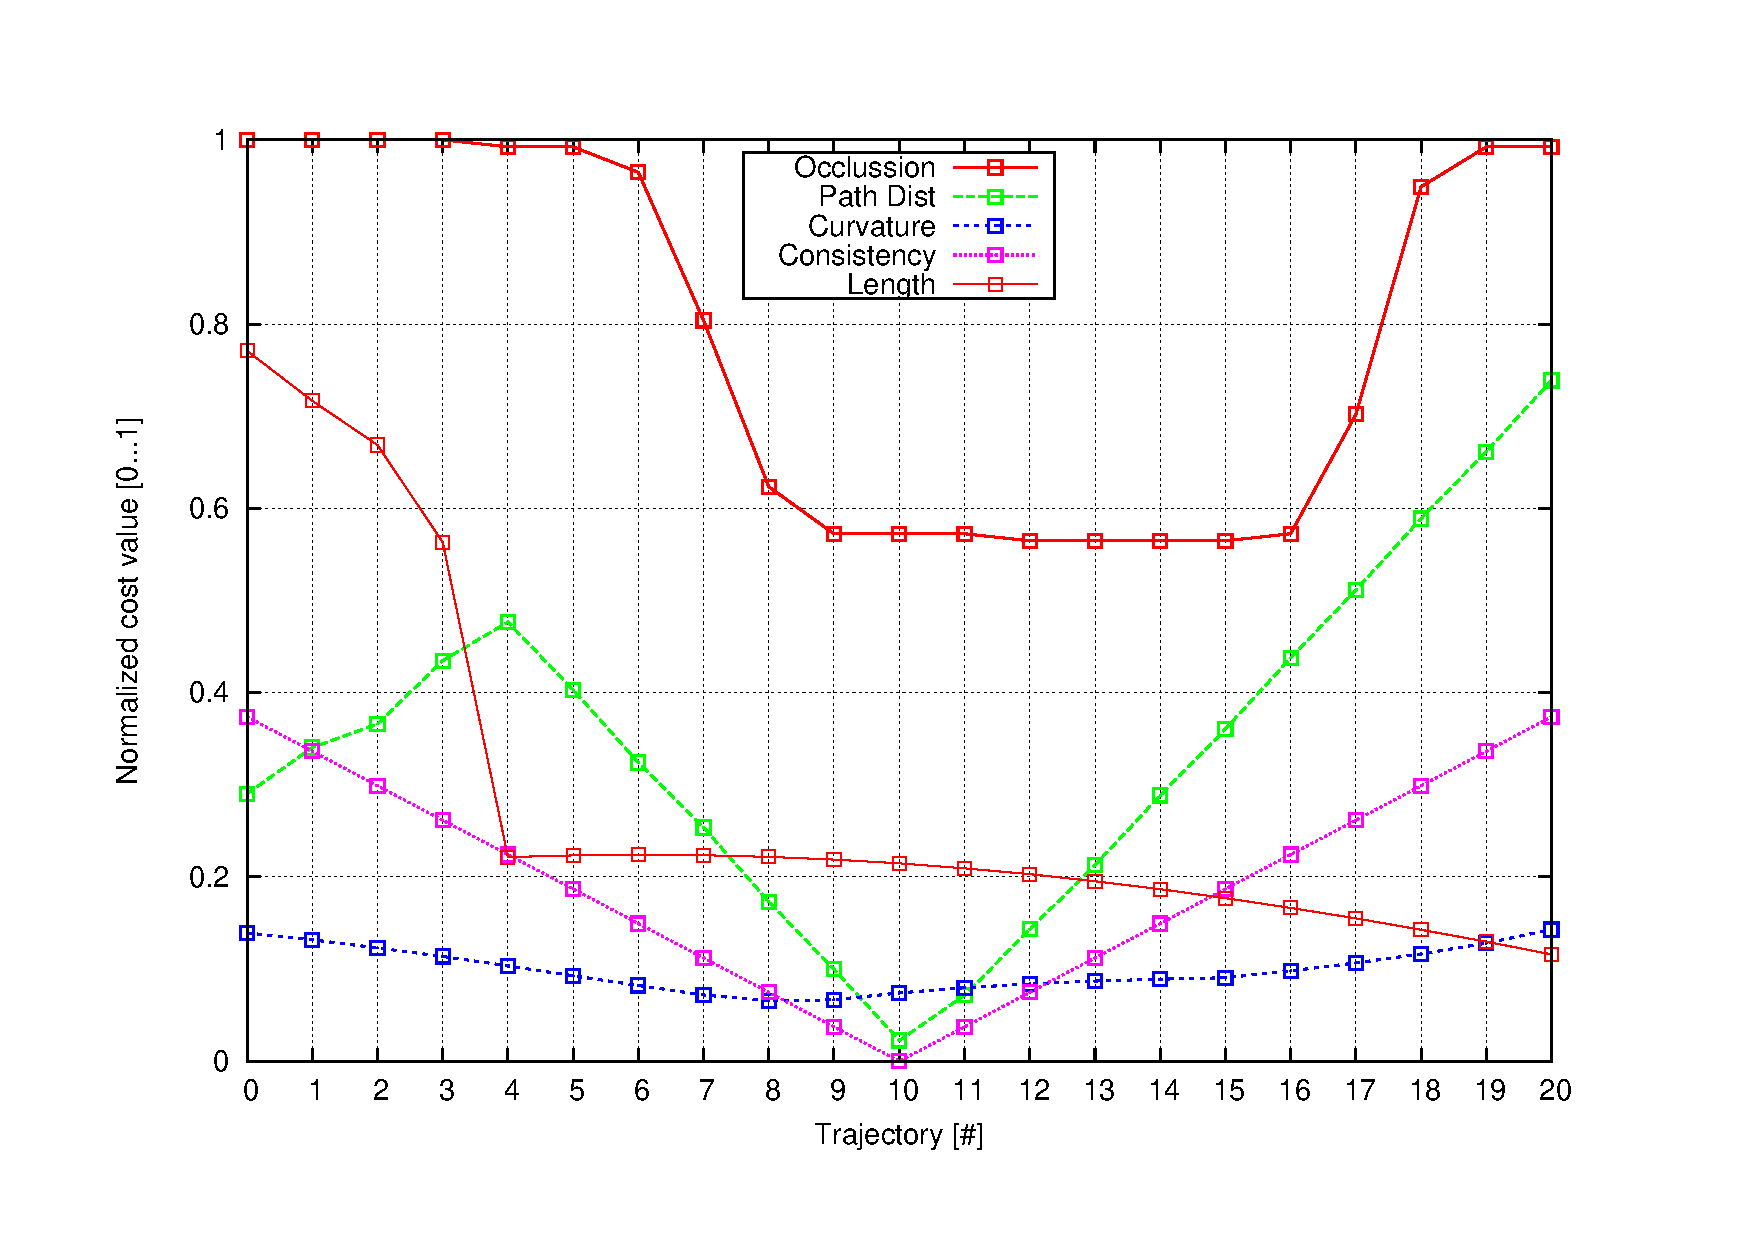
\includegraphics[width=\textwidth,trim=50 40 80 60,clip]{costs4}
    \end{center}
   \column[c]{0.5\textwidth}
    \begin{center}
      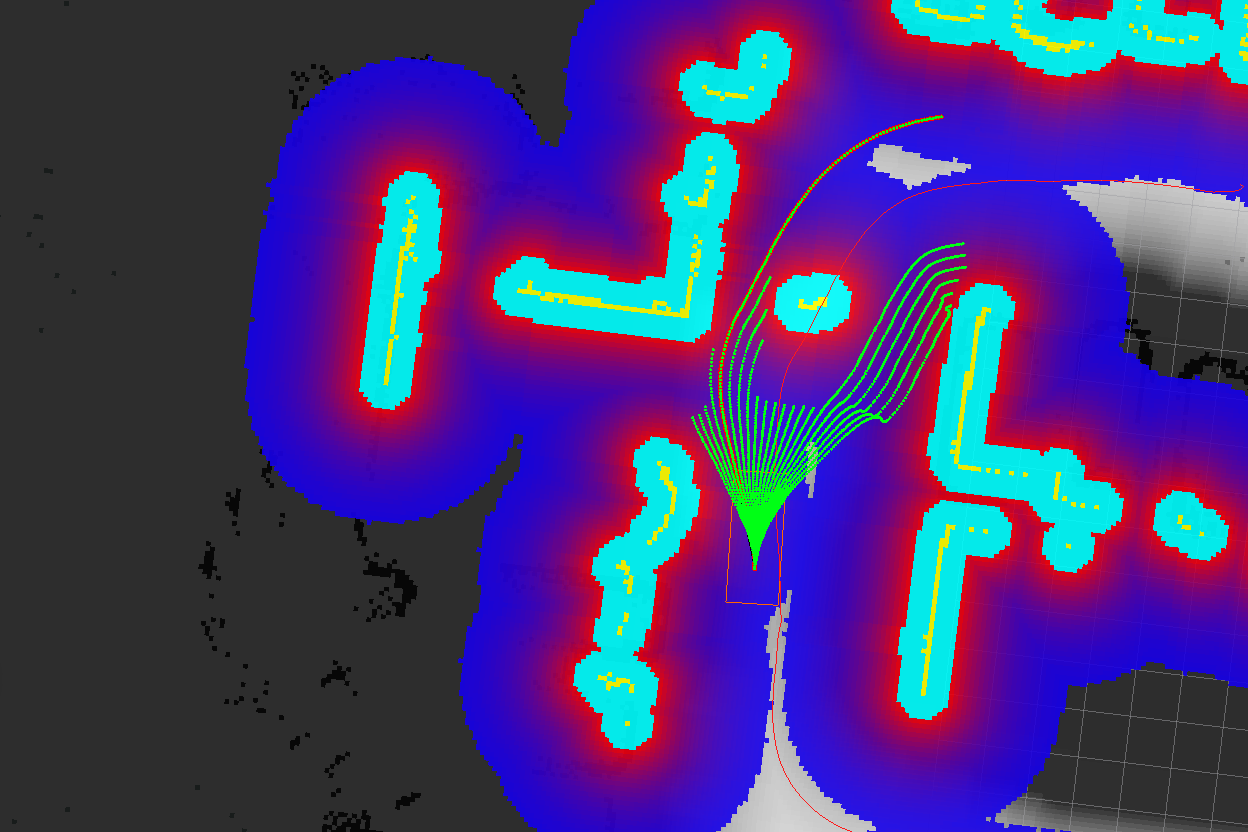
\includegraphics[width=\textwidth]{example17}\\
      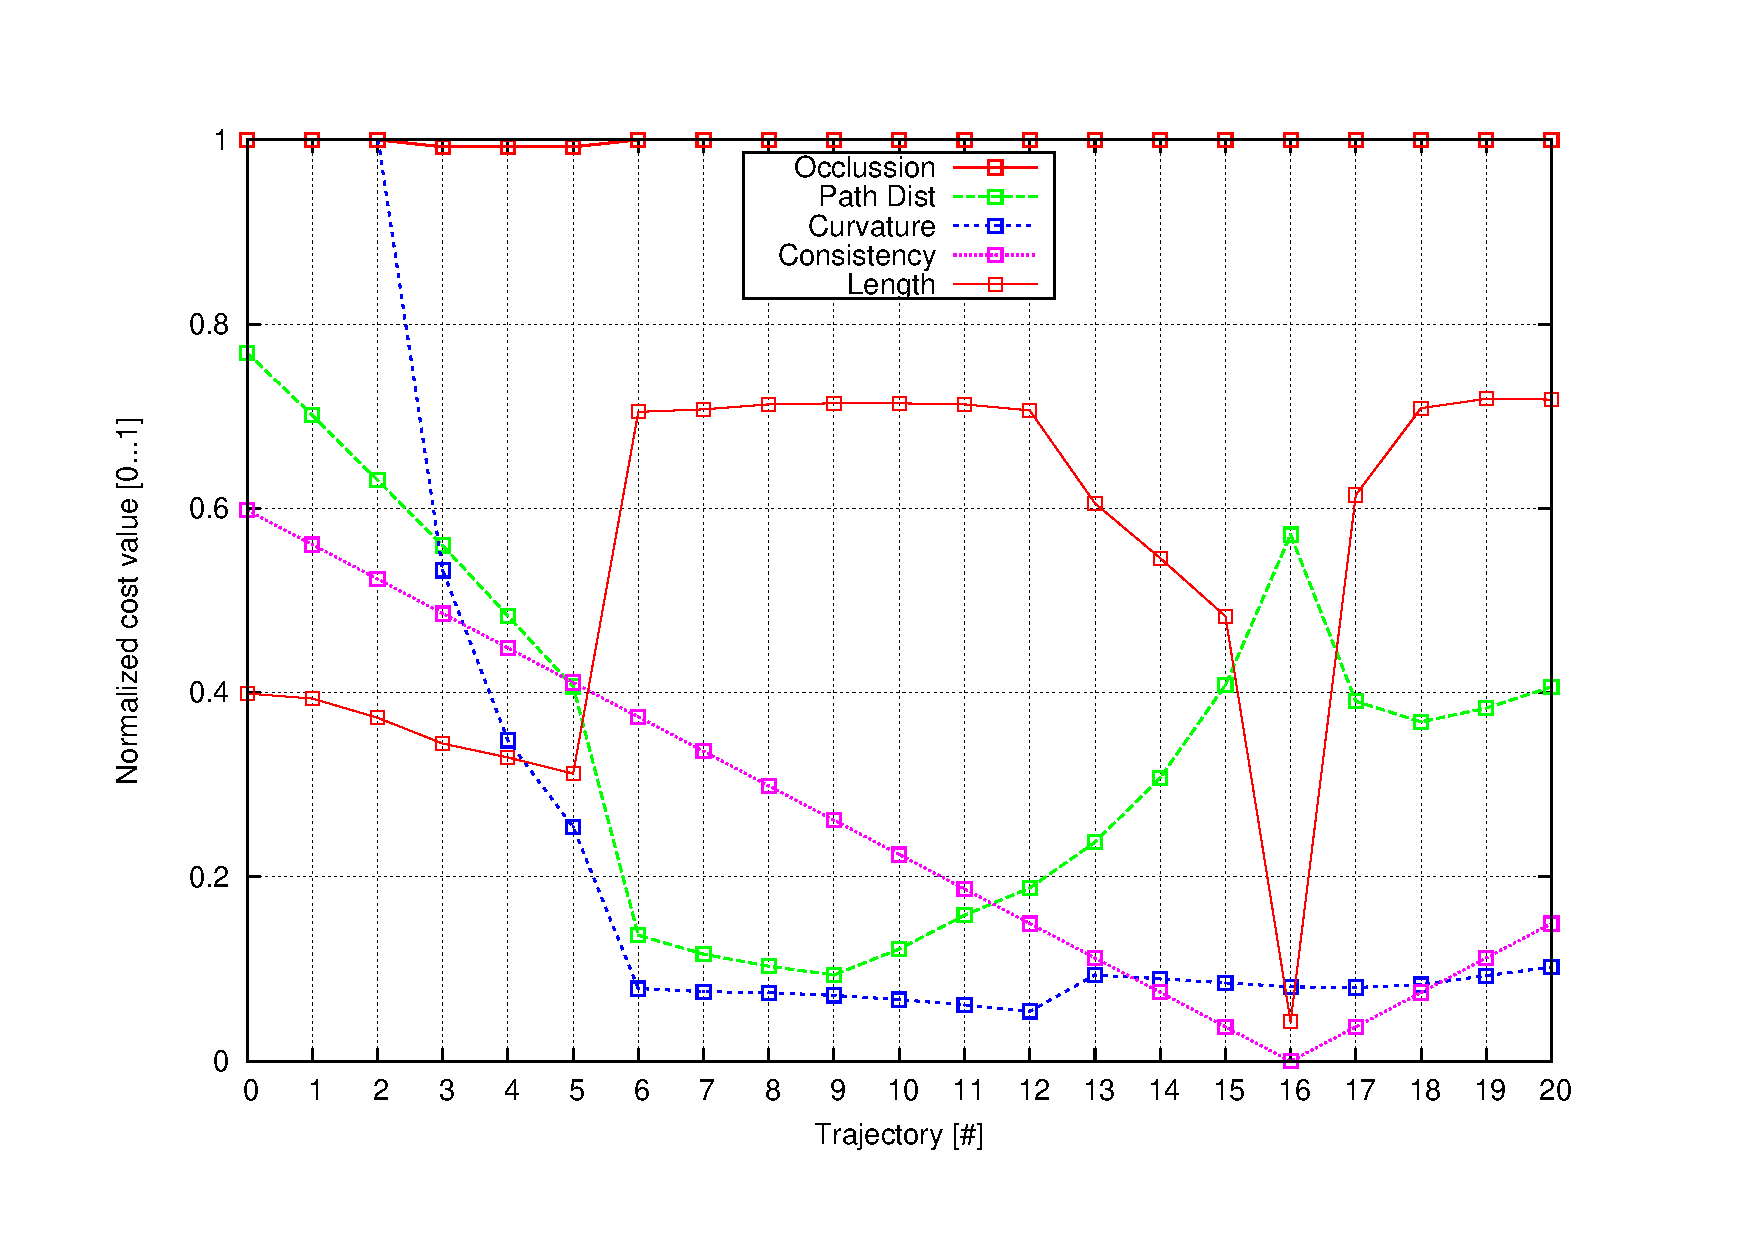
\includegraphics[width=\textwidth,trim=50 40 80 60,clip]{costs17}
    \end{center}
  \end{columns}
\end{frame}

% \begin{frame}[plain]{Obstacle avoidance}
%   \begin{columns}
%    \column[c]{0.5\textwidth}
%     \begin{center}
%       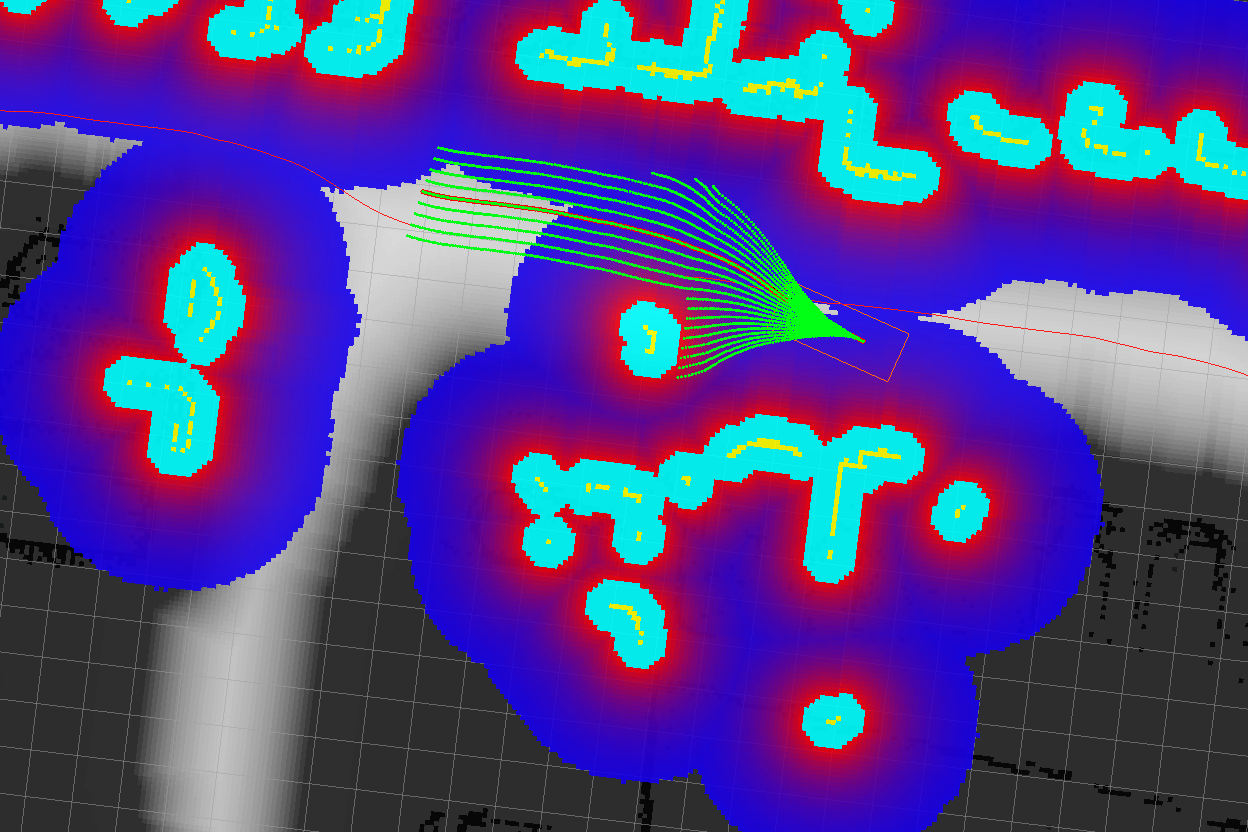
\includegraphics[width=\textwidth]{example10}\\
%       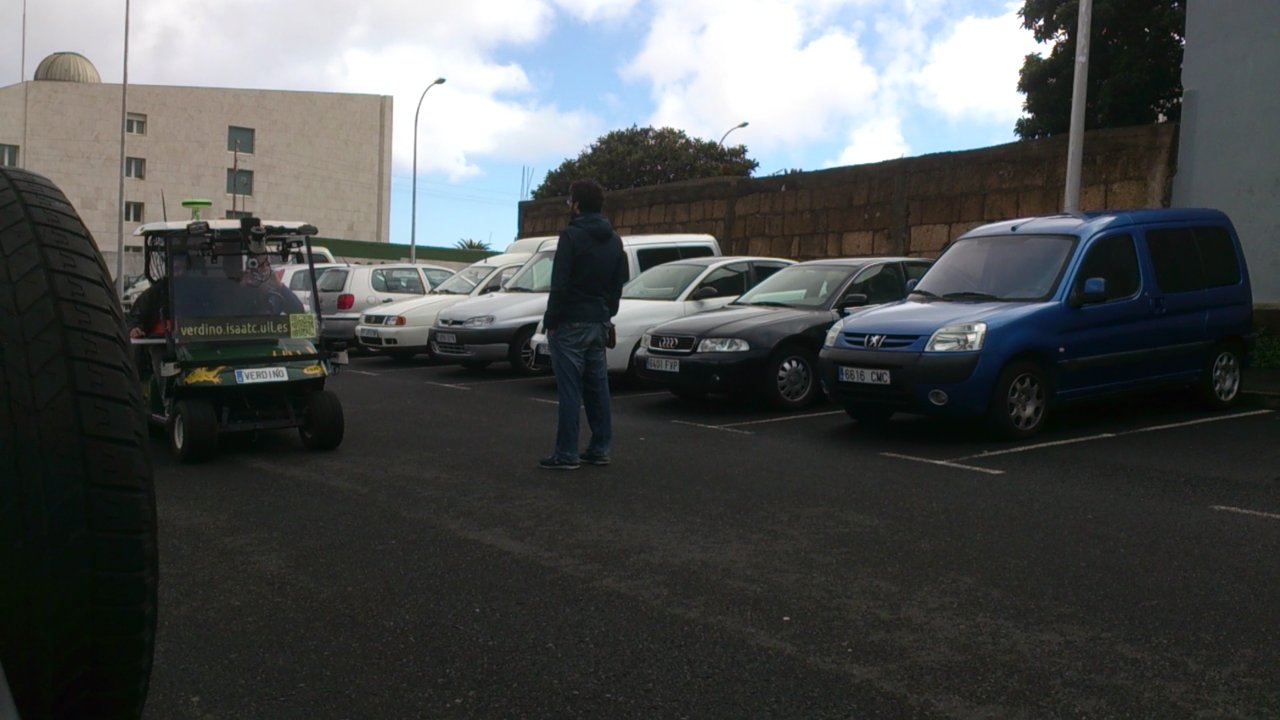
\includegraphics[width=\textwidth]{seq10}
%     \end{center}
%    \column[c]{0.5\textwidth}
%     \begin{center}
%       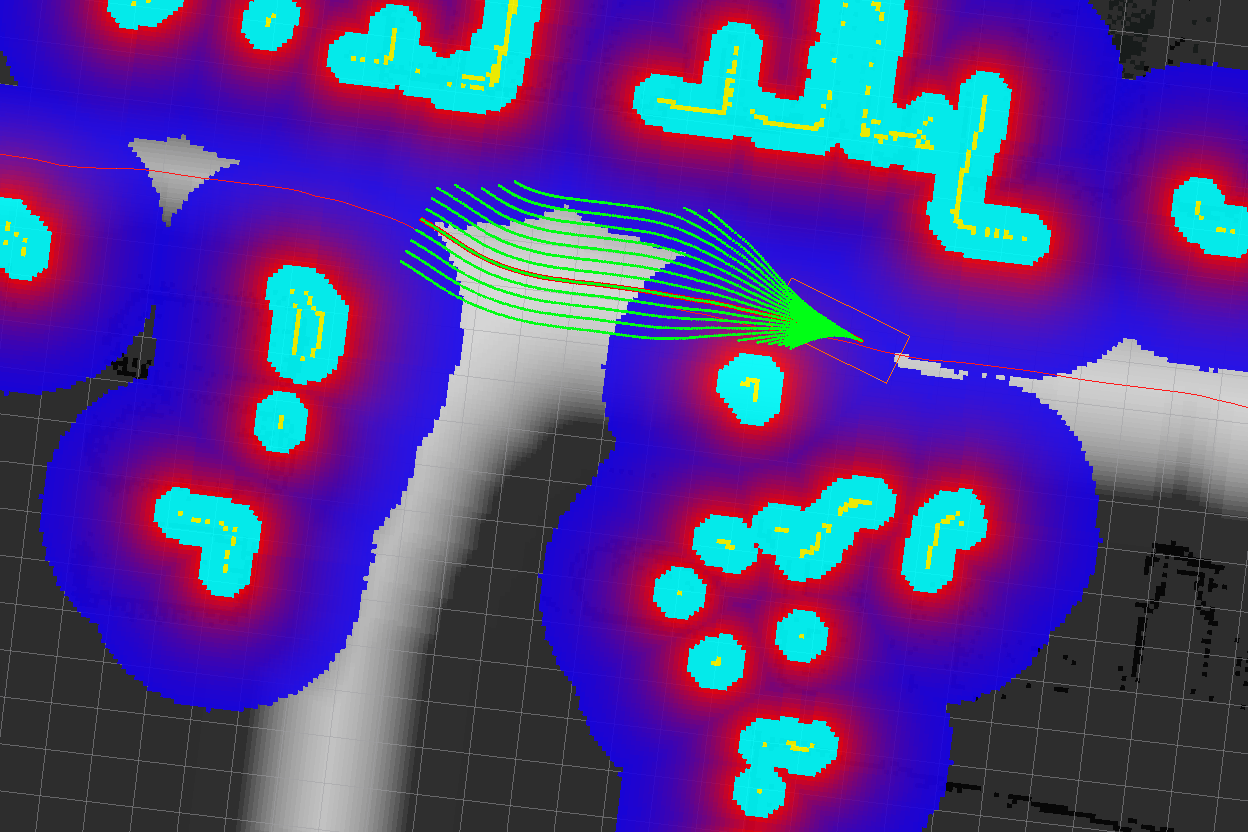
\includegraphics[width=\textwidth]{example11}\\
%       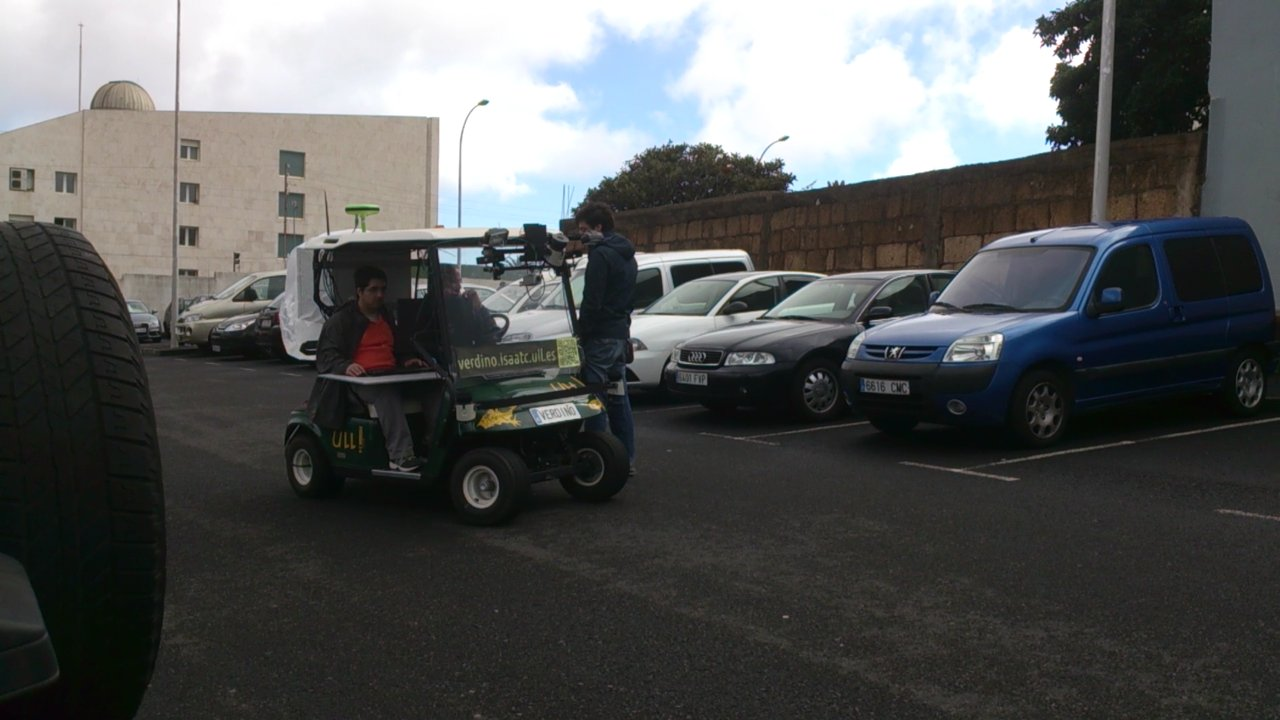
\includegraphics[width=\textwidth]{seq11}
%     \end{center}
%   \end{columns}
% \end{frame}

\begin{frame}[plain]{Putting all together}
  \begin{columns}
   \column[c]{0.5\textwidth}
    \begin{center}
      Stixel world\\~\\
      \includemovie[autoplay, repeat, controls]{\linewidth}{.75\linewidth}{/home/nestor/Seafile/Videos/Tesis/cp07/stixelsNavigation.mp4}
    \end{center}
   \column[c]{0.5\textwidth}
    \begin{center}
      Particle filter based\\~\\
      \includemovie[autoplay, repeat, controls]{\linewidth}{.75\linewidth}{/home/nestor/Seafile/Videos/Tesis/cp07/pfNavigation.mp4}
    \end{center}
  \end{columns}
\end{frame}